\documentclass[logo,ejecucion]{tesis-postgrado}
% * <laiglesiaesunnegocio@gmail.com> 2015-02-19T18:34:16.944Z:
%
%
%
% opciones: logo,dosguias,magister,doctorado,propuesta,txfonts

%\keywords{Desktop Grid; Javascript; Node.js; Volunteer Computing}

\begin{document}
\baselineskip 23pt

\frontmatter %Utiliza numeración romana

% ----------------------------------------------------------
% ----------- PARTE INICIAL --------------------------------
\thispagestyle{empty}
% Rellenar con la informacion personal y del trabajo

\titulo{Herramienta de dise\~no de objetos y visualizaci\'on de resultados para simulaci\'on de campo magn\'etico}

\autor{Juan Pablo Verdejo Jorquera}
\run{17190723-3}
\email{juan.verdejo@usach.cl}
\annoingreso{2015}

\fecha{Viernes}{05}{Junio}{2015}

\profesorguia{Fernando Rannou, Ph.D.}
\ciudad{Santiago}
\pais{Chile}

\makecubierta

\paginaenblanco


% ----------------------------------------------------------
% ----------- PRIMERA PARTE --------------------------------
% ### Resumen e Indices ####
\pagestyle{fancy}
\renewcommand{\headrulewidth}{0pt} %Hace que no aparezca la linea horizontal superior al principio de estas páginas
\fancyhead[L]{}
\fancyhead[C]{}
\fancyhead[R]{}

%\fontsize{10}{12} %Tamaño de fuente por defecto en 10pt
\linespread{1.5} %interlineado de 1.5 para el documento
\normalsize %Tamaño 10 para el cuerpo de la tesis

\makecopyright % si es propuesta no se mostrará

\resumenCastellano{
La flexibilidad sintáctica, y el complejo anidamiento de los datos en una estructura tipo árbol 
dificulta expresar propiedades deseables de los datos XML, ofreciendo una capacidad limitada para 
expresar semántica. En esta tesis se presenta un estudio de las claves como restricciones de 
integridad sobre documentos XML, implementando algoritmos para los problemas de implicación y 
validación, con el fin de mostrar la factibilidad de usar las capacidades semánticas que éstas 
entregan, y que XML como modelo requiere.
\vspace*{0.5cm}
\KeywordsES{XML; Claves XML; Implicación de claves; Validación de documentos XML; Cover no redundante}
}

\newpage

\resumenIngles{
The syntactic flexibility and complex tree-like nested data make it challenging to express desirable 
properties of XML data, offering a limited capability to express semantic. In this thesis, we present 
a study of keys as integrity constraints on XML documents, implementing algorithms for implication 
and validation problems, with the aim of showing the factibility of using the semantic capabilities 
that keys gives and XML as a model requires.
\vspace*{0.5cm}
\KeywordsEN{XML; XML keys; Key implication; XML document validation; Non-redundant cover}
}


\dedicatoria{
  A mi\ldots
}

\begin{agradecimiento}
Agradezco a ...blablabla
\end{agradecimiento}


\pagestyle{fancy}
%\fancyhead[L]{\slshape \leftmark}


\tableofcontents        %% Indice general
\newpage
\listoftables           %% Indice de tablas
\newpage
\listoffigures          %% Indice de figuras
\newpage
%\listofalgorithms       %% Indice de algoritmos



% ----------------------------------------------------------
% ----------- SEGUNDA PARTE --------------------------------
\mainmatter %Reinicia el contador de páginas para partir de 1 y usando números arábicos.
% ### Configuración del header ###
\pagestyle{fancy}
\renewcommand{\headrulewidth}{0.4pt} %Hace que vuelva a aparecer la linea horizontal

%\fancyhead[LE,RO]{\slshape \leftmark} %Hace que se muestre el título del capítulo en las páginas que no son la primera de cada capítulo
%Comentar la linea anterior y descomentar la siguiente si se usa oneside:
\fancyhead[L]{\slshape \leftmark}

%espacio entre parrafos en el cuerpo de: 3mm extras
\setlength{\parskip}{3mm}

% ### Capitulos de la tesis ###
\chapter{Introducci\'on}
\label{cap:intro}

\section{Antecedentes y motivaci\'on}
\label{intro:motivacion}

Investigadores del Departamento de Física de la Universidad de Santiago de Chile pertenecientes al Centro para el Desarrollo de la Nanociencia y la Nanotecnología (CEDENNA) trabajan en la simulación de los efectos del campo magnético en los átomos de distintos objetos, tomando en cuenta su forma, su material y su distribución atómica, entre otras características.

La simulación consiste en ejecutar eun programa computacional que implementa el Método Monte Carlo Cadenas de Markov (MCMC, \emph{Monte Carlo Markov Chain}) sobre una grilla tridimensional de átomos. Uno de los grandes problemas de los usuarios de este software es que el proceso previo y posterior a la simulación es ``manual''. Para definir el objeto a simular deben hacer un dibujo en Microsoft Paint\textregistered, el cual es analizado por un \emph{script} de Matlab\textregistered\ que debe ser modificado para reflejar las características del objeto específico que se quiere simular. Para generar imágenes para, por ejemplo, una publicación, también deben ejecutar ciertos \emph{scripts}, sin embargo esto es aún más complicado, ya que deben hacer ensayo y error hasta conseguir que la imagen sea representativa del resultado, puesto que muchas veces tienen errores de visualización que no reflejan el estado real del sistema. Estos dos sub-procesos hacen que el proceso de simulación sea tedioso, quitando mucho tiempo que podría ser usado en analizar los resultados.

Es aquí donde la informática puede contribuir, creando aplicaciones que mejoren estos procesos, que valoricen el tiempo de los científicos. Por consiguiente esta es una oportunidad única de ayudar a la obtención de conocimientos que permitan entender el entorno y de mejorar los procesos que permiten avanzar como sociedad hacia la comprensión del universo.


\section{Descripci\'on del problema}
\label{intro:problema}

El proceso actual de diseño de estructuras atómicas a simular y su visualización ha sido creado por distintos investigadores que han sido parte del CEDENNA, los cuales en general solo tienen conocimientos básicos de diseño y desarrollo de software, esto ha llevado a que este proceso se base mayoritariamente en \emph{scripts} de \emph{MatLab}, los que deben ser modificados y ejecutados manualmente para ir obteniendo los resultados deseados, esto resulta en la posibilidad de que los usuarios introduzcan errores fácilmente, los que pueden ser muy difíciles de detectar debido a la mala calidad de las pre-visualizaciones que se logran. Debido a la naturaleza de esta solución se requiere de un prolongado periodo de tiempo para poder generar datos para las simulaciones.

Una vez ejecutada la simulación es necesario poder visualizar los resultados de esta, para lo cual también se basan en \emph{scripts} de \emph{MatLab}, los que después de un largo proceso, debido a las distintas configuraciones manuales que deben hacer, genera imágenes de calidad pobre para publicaciones. Esto genera una gran pérdida de tiempo para los investigadores.

A continuación se describe con más detalle el proces actual que los investigadores realizan.


\section{Proceso actual}

\subsection{Diseño de objetos para simular}

Actualmente los científicos no tienen un proceso definido y formal de creación de objetos para simulación, ya que existen diversas soluciones implementadas a través del tiempo, desde \emph{scripts} escritos en \emph{MatLab} que fueron creados especialmente para diseñar un objeto en específico hasta unos \emph{scripts} más genéricos, pero igualmente engorrosos, usando como base un mapa de bits.


\subsubsection{Diseño programático de objetos}

La primera opción para diseñar objetos es de manera programática, es decir, escribiendo un \emph{script} que defina todas las partículas de un objeto y sus vecindades. Para alguien con experiencia en esta área puede ser relativamente sencillo diseñar algunos objetos regulares, como por ejemplo un cilindro, no obstante el proceso se complica si se quieren diseñar estructuras irregulares. Dado que la visualización del objeto diseñado es de muy baja calidad con este sistema es fácil cometer errores que eventualmente pueden invalidar los resultados de una simulación.

La figura \ref{procesoactualacript} muestra un ejemplo de la visualización de un \emph{script} de MatLab que genera un cilindro con radio $R = 60nm$ y altura $H = 20nm$ escalado a un sistema con solo 4 capas de átomos.

\begin{figure}[ht]
  \centering
  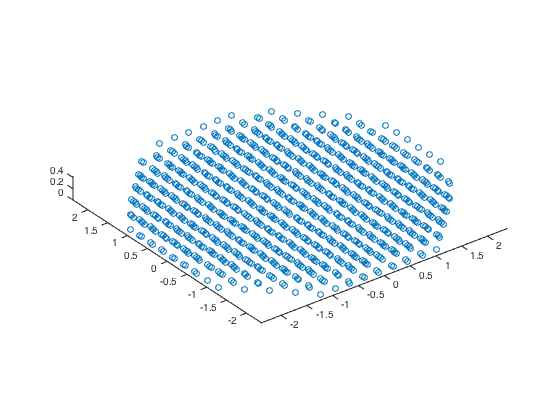
\includegraphics[scale=.6]{images/procesoActualScript}
  \caption{\em Ejemplo de imagen salida de un \emph{script} de generación de objeto}
  \label{procesoactualacript}
\end{figure}

\subsubsection{Diseño en base a mapa de bits}
\label{intro:procesoactualmapa}

Para flexibilizar el diseño de objetos y bajar la posibilidad de introducir errores en los datos de entrada se creó un sistema que permite especificar la geometría de un objeto en base a un mapa de bits construido en \emph{Microsoft Paint}. De esta forma no es necesario escribir un progama cada vez qe se cambiase la geometría del objeto, si no que basta con crear una imagen que representa la primera capa del objeto y usar el \emph{script} de \emph{MatLab} para el tipo de estructura cristalina específica que se desea definir.

\begin{figure}[ht]
  \centering
  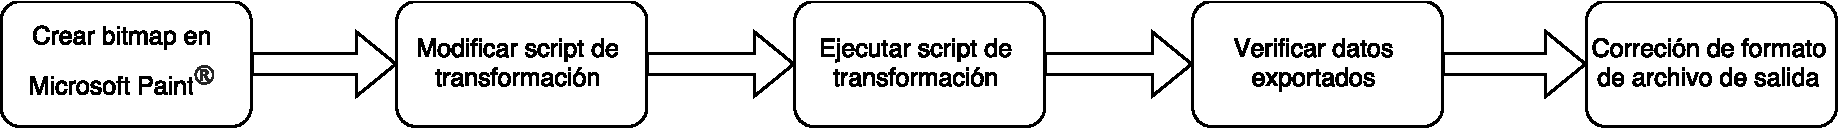
\includegraphics[scale=.5]{images/procesoActualBitmapFlujo}
  \caption{\em Flujo para creación de diseño de objetos en base a mapa de bits}
  \label{procesoActualBitmapFlujo}
\end{figure}

Como se puede ver en la figura \ref{procesoActualBitmapFlujo}, para iniciar este proceso es necesario tener un editor de imágenes que permita crear archivos .bmp, como por ejemplo Microsoft Paint\textsuperscript{\textregistered}. Con este editor se crea una imagen del tamaño y forma deseada, la cual usualmente no excede los 50px x 50px. Luego se debe pintar, con color negro, los pixeles que representen la primera capa de átomos del objeto. Estos pixeles luego serán identificados por un \emph{script} de \emph{Matlab}, como posiciones relativas de átomos del objeto.

En la figura \ref{procesoActualBitmap} siguiente imagen se muestra un ejemplo de estos mapas, usando una imagen de 10px x 10px. Esta figura solo representa la forma y posiciones relativas de los átomos y no considera el tipo de átomo ni la estructura cristalina que ellos forman.

\begin{figure}[ht]
  \centering
  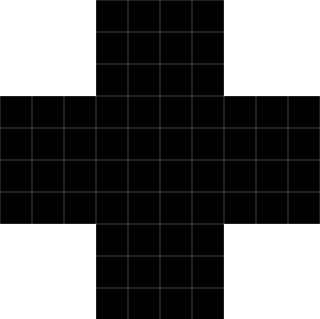
\includegraphics[scale=.6]{images/procesoActualBitmap}
  \caption{\em Mapa de bits de 10px x 10px}
  \label{procesoActualBitmap}
\end{figure}

Para introducir esta información se debe modificar otro \emph{script} de \emph{Matlab}, el cual tiene múltiples versiones según el tipo de estructura cristalina que se quiera diseñar, que agrega los parámetros físicos del objeto. Algunas de las opciones que se deben configurar antes de iniciar la ejecución son:

\begin{description}
	\item [Número de capas] \hfill \\
		Cuántas veces se repite la primera capa para formar un objeto en 3D.
	\item [Coeficiente de escalamiento] \hfill \\
		Es un coeficiente usado para dar al objeto las medidas deseadas para ejecutar la simulación.
	\item [Constante de red] \hfill \\
		Esta es la dimensión real (en nanómetros) de la arista de una celda unitaria
\end{description}

Todos estos parámetros deben ser modificados directamente en el código, y en distintas partes de este, por lo que es muy fácil cometer errores, los que por supuesto invalidan cualquier simulación hecha en base a estos.

Una vez configurado el script, este debe ser ejecutado. Se lee el mapa de bits ingresado como parámetro analizando cada uno de los pixeles, creando un arreglo binario de 2 dimensiones, donde un pixel negro es representado por un 1 y un pixel blanco es representado por un 0, lo que creará la primera capa de átomos; luego, según las configuraciones ingresadas, generará el resto de átomos buscados con sus correspondientes vecinos. El resultado es un archivo con las posiciones de los átomos y sus vecinos, además de dos imágenes que representan las distintas partículas generadas en base a los archivos de entrada. Estas imágenes no son lo suficientemente claras como para poder identificar errores en el diseño esperado, por lo que la posibilidad de equivocarse y simular con una premisa inválida es algo mucho más común que lo esperado.

La figura \ref{procesoActualMatlab1} muestra la visualización 3D del objeto de la figura \ref{procesoActualBitmap} generado con \emph{MatLab}. Como se puede apreciar esta visualización no permite distinguir claramente la forma de cruz del objeto. Solo una vista 2D, como la de la figura \ref{procesoActualMatlab2}, permite corroborar la forma adecuada.

\begin{figure}[ht]
  \centering
  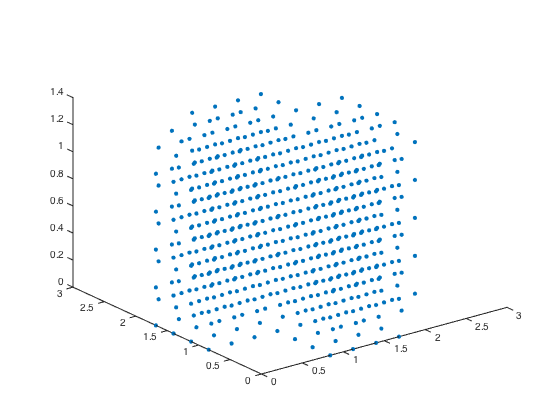
\includegraphics[scale=.6]{images/procesoActualMatlab1}
  \caption{\em Vista 3D de los átomos encontrados}
  \label{procesoActualMatlab1}
\end{figure}

\begin{figure}[ht]
  \centering
  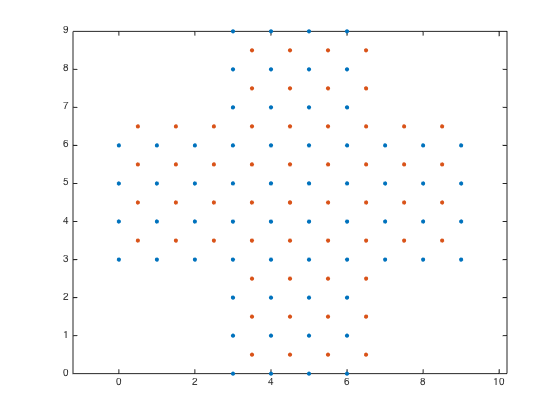
\includegraphics[scale=.6]{images/procesoActualMatlab2}
  \caption{\em Vista 2D de la primera capa de átomos}
  \label{procesoActualMatlab2}
\end{figure}

Una vez decidido que el objeto diseñado se usará para una simulación es necesario ejecutar un nuevo software, escrito en C, que se encarga de modificar el archivo de salida del script de \emph{Matlab} de tal forma de que pueda ser usado como entrada para la simulación Monte Carlo. Cabe notar que este software está compilado y no se cuenta con el código fuente de este, de tal forma que si en algún momento se necesitara modificar el formato de la entrada de la simulación este software se debería re-escribir.

La transformación consiste en modificar cada línea del archivo, con el siguiente formato:

\begin{center}
	\begin{lstlisting}
 5.4700000e+02   1.4000000e-01   1.5400000e+00   1.2600000e+00   4.0000000e+00   4.8300000e+02   4.8400000e+02   4.8700000e+02   4.8800000e+02   0.0000000e+00   0.0000000e+00   0.0000000e+00   0.0000000e+00
	\end{lstlisting}
\end{center}

\noindent
y eliminar todas las potencias, reemplazándolas, de ser posible, con números enteros. Además es necesario agregar una línea en el inicio del archivo que contiene distintos parámetros usados por el software de simulación, como el número de partículas y la constante de escalamiento.

Un ejemplo de las primeras 5 líneas de un archivo correcto sería:

\begin{center}
	\begin{lstlisting}
 104	1	8	0.00245
 1	-0.19799	-1.26	0	3	3	4	54	0	0	0	0	0
 2	0.19799	-1.26	0	3	4	5	55	0	0	0	0	0
 3	-0.39598	-1.12	0	4	1	6	7	58	0	0	0	0
 4	0	-1.12	0	6	1	2	7	8	52	59	0	0
	\end{lstlisting}
\end{center}

En la primera línea los datos necesitados son:
\label{formatoDatos}

\begin{itemize}
	\item Número de átomos descritos en el archivo
	\item $1$. Este valor no se utiliza y se mantiene por razones de compatibilidad con antiguas versiones del software de simulación
	\item Número máximo de vecinos
	\item Constante de escalamiento
\end{itemize}

Desde la segunda línea en adelante el formato es:

\begin{itemize}
	\item ID del átomo
	\item Componente $\hat{i}$ de la ubicación
	\item Componente $\hat{j}$ de la ubicación
	\item Componente $\hat{k}$ de la ubicación
	\item Cantidad de vecinos del átomo
	\item ID del vecino 1
	\item ID del vecino 2
	\item ...
	\item ID del vecino N
\end{itemize}

En caso de que un átomo tenga un número vecinos inferior al máximo posible se deben rellenar la línea con ceros, de tal forma que cada línea tenga la misma cantidad de valores.

\subsection{Visualización de resultados}

Si bien el proceso de diseño de objetos es precario, este no se compara con el de visualización y exportación de resultados, tanto en forma de imágenes como videos. Dentro de las limitaciones actuales está la imposibilidad de generar videos con colores que permitan distinguir una tercera dimensión.

Actualmente se usa la funcionalidad \emph{Quiver plot} de \emph{MatLab}, que permite dibujar rápidamente vectores en base a archivos de entrada con cierto formato, no obstante este proceso requiere de tiempo para obtener representaciones que realmente reflejen lo deseado, siendo un proceso de ensayo y error que utiliza tiempo de manera innecesaria para los científicos.


% Actualmente los investigadores deben preparar la simulación usando un \emph{script} en Matlab\textregistered, el cual analiza un archivo \emph{.bmp} creado en \emph{Microsoft Paint\textregistered}, esta imagen generalmente es pequeña, menor a 50px x 50px, y representa la primera capa del objeto (mirado desde arriba), para esto se marcan los pixeles que describen el objeto, de esta forma el mapa de \emph{bits} es binario, si un \emph{pixel} es negro se considera un 1, si es blanco se considera un 0. En este \emph{script} se describen características específicas del objeto que se quiere definir, entre ellos:
% \begin{itemize}
% 	\item Número de capas: Cuantas veces se repite la primera capa para formar un objeto en 3D.
% 	\item Distribución de los átomos (ver anexo A): Como premisa se trabaja sólo con distribuciones cúbicas de átomos, no obstante estas distribuciones tienen ciertas características específicas, por ejemplo:
% 	\begin{itemize}
% 		\item Cúbico simple (SC por \emph{Simple Cubic}): En cada vértice de una distribución cúbica se encuentra un átomo.
% 		\item Centrado en las caras (FCC por \emph{Face-centered Cubic}): Además del átomo en cada vértice de la distribución cúbica, hay un átomo en el centro de cada cara de la distribución.
% 		\item Centrado (BCC por \emph{Body-centered Cubic}):  Además del átomo en cada vértice de la distribución cúbica, hay un átomo en el centro de cada distribución.
% 	\end{itemize}
% 	\item Coeficiente de escalamiento: Es un coeficiente usado para dar al objeto las medidas deseadas para ejecutar la simulación.
% \end{itemize}

% Este proceso produce un archivo de texto plano describiendo cada uno de los átomos del objeto sobre el cuál se aplicará la simulación.

% Luego de ejecutada la simulación el software entrega múltiples archivos de texto, uno que define cada uno de los átomos con un ID y una posición en el espacio, y N archivos que definen la fuerza magnética de cada átomo en un tiempo dado. Los científicos deben seleccionar uno de estos archivos y aplicar un \emph{script} de Matlab\textregistered\ para poder visualizar el resultado.

% El proceso de exportación de imágenes para publicaciones puede tomar un día de trabajo para los científicos, ya que deben hacer ``ensayo y error'' hasta que la imagen producida refleje lo que desean. Luego deben esperar por la aprobación por parte del profesor guía, en caso de ser rechazada, deben volver a ejecutar el proceso.

% \subsection{Soluciones similares}
% Existe una herramienta que hace simulaciones similares a las que hace el grupo de científicos llamada ``Go Parallel Magnet\textregistered''. A pesar de que la simulación no es exactamente la misma, el flujo de diseño es útil para el proyecto. Sin ir más lejos los científicos basan el proceso actual en éste.

% ``Go Parallel Magnet\textregistered'' usa para el diseño un sistema de multi-capas, donde se define la capa superior del objeto y se indica la cantidad de veces que ésta se repetirá. Con estos datos se crea un objeto en 3D que luego se transforma en la estructura molecular deseada.

\section{Propósitos de la solución}
\begin{enumerate}
  \item Automatizar el proceso de diseño de configuraciones atómicas usadas para la simulación, de forma de disminuir tanto el tiempo requerido para esto como la probabilidad de introducir errores humanos, los que pueden inválidar una simulación
  \item Permitir el manejo interactivo durante el diseño de una configuración atómica mediante rotaciones, traslaciones y \emph{zoom}
  \item Exportar configuraciones atómicas que puedan ser simuladas inmediatamente, sin necesidad de transformar los datos
  \item Generar imágenes de alta calidad para publicaciones, tanto de una configuración atómica diseñada como de un estado de la simulación en un tiempo $t$
  \item Generar videos de cambios de estados de una simulación para presentación en conferencias
\end{enumerate}


\section{Alcances o limitaciones de la solución}
\begin{itemize}
	\item El software se encargará del diseño de objetos para la simulación entregando la entrada para ésta y posteriormente de la visualización de los resultados, y de la exportación de estos para publicaciones, mas no se encargará de la simulación en sí, la cual queda fuera del alcance de la solución.
	\item La aplicación estará disponible para sistema operativo MAC OS X.
	\item El diseño de objeto será por capas, es decir, se define la ``vista superior'' y la cantidad de veces que se repetirá hacia abajo.
\end{itemize}

\section{Objetivos y alcance del proyecto}
\label{intro:objetivos}

\subsection{Objetivo general}
Diseñar e implementar una aplicación para el diseño interactivo de configuraciones atómicas 3D, basado en capas, y para la visualización dinámisa y estática de la evolución de dicha configuración durante una simulación de campo magnético.

\subsection{Objetivos espec\'ificos}

Para la consecución del objetivo general, se plantean las siguientes metas intermedias para el proyecto:

\begin{enumerate}
  \item Definir los requerimientos funcionales, en base a la interiorización en el proceso actual de los investigadores
  \item Diseñar los componentes de diseño de configuraciones atómicas y visualización de resultados de la simulación
  \item Construir los componentes utilizando las herramientas de desarrollo mencionadas en el punto \ref{herramientasdesarrollo}
  \item Probar la aplicación
\end{enumerate}


\section{Características de la solución}

Como solución se propone la creación de un software que facilite el trabajo de los científicos. Esta aplicación se divide en dos funcionalidades:

\subsection{Diseño de configuraciones atómicas}

El software debe permitir la creación visual e interactica de un objeto en 3D, con ciertas características físicas como el tipo de estructura cristalina. Luego de la creación y configuración del objeto, la aplicación debe exportar un archivo de texto que sirva como entrada para el software que realiza la simulación. Este archivo tiene un formato expecífico, el cual fue definido en el punto \ref{formatoDatos}.

\subsection{Visualización dinámica de la evolución de las configuraciones atómicas}

El software debe tomar la totalidad de archivos de salida de la simulación como entrada y debe ser capaz de mostrar visualmente el estado magnético de cada átomo en un tiempo $t$. También debe ser posible ver la simulación animada a través del tiempo, como un video.

La salida de la visualización serán imágenes en 2D del estado de la simulación en un tiempo $t$. Estas imágenes deben tener colores que permitan al lector entender el resultado a pesar de la dimensión faltante, por ejemplo, usando la proyección del vector en uno de los ejes y asignando un color según la intensidad de éste.


\section{Metodolog\'ia y herramientas utilizadas}
\label{intro:metodologia}

\subsection{Metodolog\'ia}
Dado que se tiene conocimiento de los requerimientos mayores, pero pueden existir detalles al trabajar en un ámbito tan específico como simulaciones físicas, se decidió usar una modificación de la metodología Scrum \citep{SCRUM}.

Scrum está pensado para trabajar en equipos con varios desarrolladores, además de los cargos de gestión, para lo cual se tienen 3 roles \citep{website:ScrumRoles}:

\begin{description}
  \item[\emph{Product Owner}] \hfill \\
  Es el encargado de maximizar el valor del trabajo del equipo. Tiene un alto conocimiento del producto mediante un contacto directo con los \emph{stakeholders} y facilita la comunicación de estos con el equipo de desarrollo. Pot lo tanto es el responsable de decidir qué se va a construir, pero no el cómo. Para este proyecto el \emph{Product Owner} será el profesor Fernando Rannou, quién tiene contacto constante con los \emph{stakeholders} por proyectos paralelos que se están desarrollando.
  \item[\emph{Scrum Master}] \hfill \\
  Es el líder del equipo de desarrollo y debe tener un buen conocimiento de la metodología \emph{Scrum}, el cual debe traspasar al equipo de desarrolladores. Sus 3 principales tareas son: Guíar al equipo teniendo un conocimiento tanto del producto como de las tecnologías a utilizar; mantener al equipo avanzando eliminando toda dificultad que puedan tener durante el desarrollo (ya sea interna como externa), y enseñar la metodología \emph{Scrum} al equipo. En este caso, como el equipo de desarrollo está compuesto por sólo un desarrollador y este tiene un gran conocimiento de la metodología gracias a sus años de experiencia laboral usándola, el rol de \emph{Scrum Master} no se usará.
  \item[Desarrollador] \hfill \\
  El desarrollador es el encargado de entregar los incrementales del producto, para lo cual se basa en la lista de tareas definidas por el \emph{Product Owner} al inicio de un \emph{sprint}. En este proyecto solo trabajará un desarrollador.
\end{description}

Otras adaptaciones hechas a la metodología fue la modificación alguna de sus ceremonias, cambiando la reunión diaria (\emph{Daily Scrum}) por una semanal, entre el profesor y el desarrollador. Las reuniones retrospectivas al finalizar cada \emph{sprint} se unieron con la de planificación del siguiente periodo de desarrollo. Además, como es recomendado, se tuvo una reunión con los \emph{stakeholders} luego de cada \emph{sprint}.

Estas modificaciones fueron necesarias para poder usar la metodología en un proyecto con solo un desarrollador y optimizando al máximo el tiempo usado en reuniones, debido al poco espacio en las agendas tanto del desarrollador como del \emph{Product Owner}.

\subsection{Herramientas de desarrollo}
\label{herramientasdesarrollo}
\subsection{Modelado 3D: OpenGL}
Se usa OpenGL como biblioteca de modelado 3D, por ser el estado del arte en este ámbito. Entre sus ventajas está el ser multi-plataforma, lo que eventualmente permitiría una rápida portación a otro sistema operativo, y el ser la más usada actualmente, lo que permite que tenga una amplia comunidad de usuarios que la soportan y documentan.

\subsection{Lenguaje de programación: Python}
Para el desarrollo se usará el lenguaje de programación Python con la biblioteca wxPython para Intefaz de Usuario. Esta biblioteca tiene soporte para la API OpenGL. Python, al ser un lenguaje multiplataforma, permitiría una rápida portación a otro sistema operativo en el futuro.

\subsection{Control de versiones: GIT}
Para el versionamiento del código se usará GIT, manteniendo un respaldo del repositorio con el código y la documentación en una máquina virtual con Linux ubicada en Estados Unidos.

\section{Ambiente de desarrollo}
Para el desarrollo se usará el siguiente ambiente de desarrollo:
\begin{itemize}
	\item Computador marca Apple, con una tarjeta gráfica que soporte OpenGL 3.2+ y sistema operativo Mac OS X para el desarrollo.
	\item Una máquina virtual con Linux, ubicada en Estados Unidos, para mantener un respaldo del código y de la documentación.
\end{itemize}

\chapter{Dominio de problema}
\label{cap:dominio}

\section{Problema}
Investigadores del Departamento de Física de la Universidad de Santiago de Chile pertenecientes al CEDENNA se encuentran estudiando los efectos de aplicar ciertos campos magnéticos a nano-estructuras cristalinas, con propiedades físicas definidas. Los resultados de estas simulaciones pueden ser aplicados a la producción de nuevos dispositivos magnéticos o para el grabado de datos magnético de alta densidad  \citep{asymmetricMagneticDots}.

\section{Estructuras cristalinas}
Las nano-estructuras estudiadas son de tipo cristalinas, las que pueden ser divididas en celdas unitarias de distintos tipos  según la distribución de sus átomos. Las 3 estructuras más usadas son el cubo simple (\emph{SC} o \emph{Simple Cubic}), cubo centrado en su cuerpo (\emph{BCC} o \emph{Body-centered Cubic}) y cubo centrado en sus caras (\emph{FCC} o \emph{Face-centered cubic}) \citep{ITC213}.

En las estructuras cristalinas la dimensión física de las aristas está dada por el parámetro llamado \emph{Lattice Parameter} o Parámetro de Red. Como en este caso solo se trabajará con estructuras cúbicas todas las aristas tendrán la misma dimensión, por lo que nos referiremos a este parámetro como \emph{Lattice Constant} o Constante de Red.

Para cada átomo de una estructura cristalina se puede identificar un conjunto de átomos que componen la vecindad, es decir, son los átomos que están a menor distancia de este. Dependiendo del tipo de celdas unitarias se define un algoritmo para encontrar los vecinos e identificar el número máximo de vecinos que pueden ser encontrados.

Dependiendo del tipo de estructura se puede encontrar patrones de periodicidad entre ellas, es decir, que cada cierto número de capas se repita la misma distribución de átomos.

\subsection{Cubo simple (SC)}
\label{structureSC}
Esta es la estructura cristalina más simple, donde en cada vértice podemos encontrar una partícula. Luego la distancia entre dos átomos vecinos es siempre la constante de red (ver figura \ref{SimpleCubic}). Como en cada vértice de la estructura se unen 8 celdas unitarias, cada cubo tiene $1/8$ de partícula, luego cada celda tiene $1/8 \cdot 8 = 1$ átomo en total.

En el caso del cubo simple la vecindad de cada átomo está compuesta a lo más por otros 6 átomos, los que están en dirección a cada una de las aristas que componen el vértice donde se encuentra la partícula.

El cubo simple tiene una periodicidad de 1, es decir, todas las capas tienen la misma distribución de átomos.

\begin{figure}[ht]
  \centering
  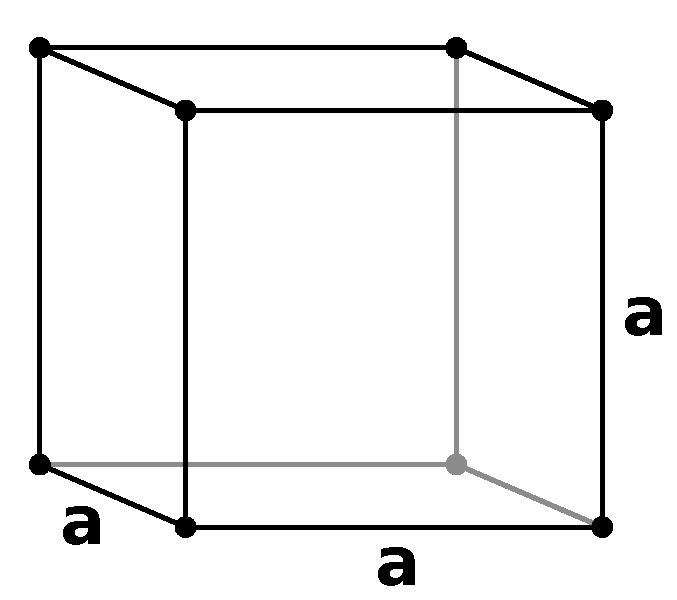
\includegraphics[scale=.6]{images/SimpleCubic}
  \caption{\em Cubo simple, con constante de red $a$}
  \label{SimpleCubic}
\end{figure}


\subsection{Cubo centrado en su cuerpo (BCC)}
\label{structureBCC}
Una estructura cristalina de cubos centrados en su cuerpo se caracteriza porque en cada una de sus celdas unitarias se puede encontrar, además de los átomos en sus vértices, un átomo en su centro (ver figura \ref{BodyCenteredCubic}). De esta forma cada una de sus celdas tiene $1/8$ de átomo en cada uno de sus vértices, más un átomo en su centro, resultando en $1/8 \cdot 8 + 1 = 2$ átomos en total.

A diferencia de un cubo simple, la vecindad de un átomo en BCC está compuesta por:

\begin{itemize}
  \item Para el caso de un átomo ubicado en un vértice, las partículas centrales de cada uno de los cubos que componen dicho vértice.
  \item Para el caso de un átomo ubicado en el centro de una celda unitaria, las partículas ubicadas en cada uno de los vértices de dicha celda.
\end{itemize}

En ambos casos el número máximo de partículas en una vecindad es de 8.

La periodicidad de capas de una estructura compuesta por cubos centrados en su cuerpo es de 2, es decir, cada 2 capas se repetirá la distribución de átomos.

\begin{figure}[ht]
  \centering
  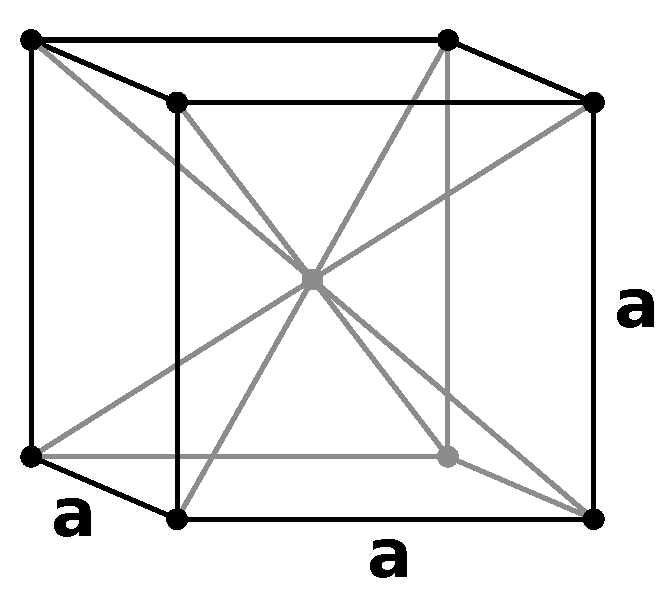
\includegraphics[scale=.6]{images/BodyCenteredCubic}
  \caption{\em Cubo centrado en su cuerpo, con constante de red $a$}
  \label{BodyCenteredCubic}
\end{figure}


\subsection{Cubo centrado en sus caras (FCC)}
\label{structureFCC}
En el caso de las estructuras cristalinas compuesta por cubos centrados en sus caras se puede distinguir átomos en cada uno de sus vértices y átomos en cada una de las caras de cada cubo (ver figura \ref{FaceCenteredCubic}). Como el átomo de una cara es compartido por 2 cubos, cada uno de ellos contiene $1/2$ de éste, y por lo tanto cada celda unitaria contiene $1/8 \cdot 8 + 1/2 \cdot 6 = 4$ átomos en total.

La vecindad de un átomo FCC está compuesta por:

\begin{itemize}
  \item Las partículas de cada cara que esté compuesta por una de las aristas que conforman el vértice, para el caso de un átomo ubicado en ese punto
  \item En el caso de las partículas que se encuentran en una cara, todos los átomos ubicados en las caras formados por las aristas que componen la cara del átomo inicial (2 caras por arista), además de los átomos que están en los vértices que componen la cara inicial
\end{itemize}

De las reglas anteriores se puede inferir que el tamaño máximo de una vecindad es de 12 átomos.

Para las estructuras formadas por cubos centrados en sus caras se identifica una periodicidad de 2, es decir, al igual que en el caso de los cubos centrados en su cuerpo, cada 2 capas se repite la distribución atómica.

\begin{figure}[ht]
  \centering
  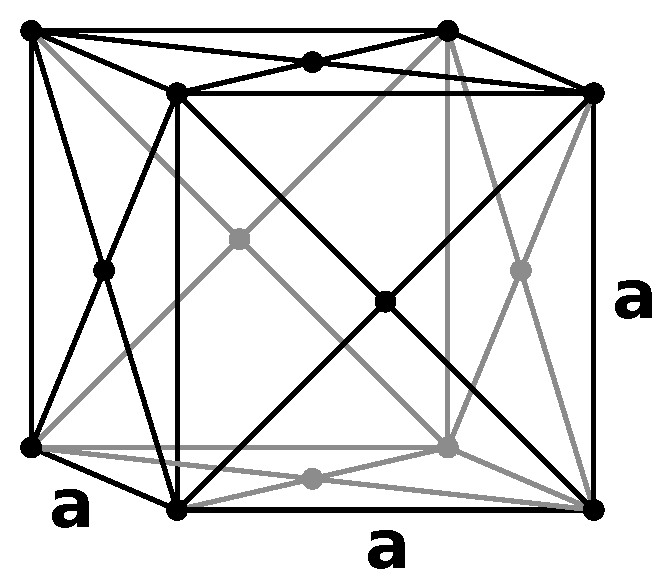
\includegraphics[scale=.6]{images/FaceCenteredCubic}
  \caption{\em Cubo centrado en sus caras}
  \label{FaceCenteredCubic}
\end{figure}

\section{Escalamiento}

A pesar de la gran capacidad de procesamiento de los computadores actuales aún resulta inconveniente simular los sistemas con sus características reales, debido a la gran cantidad de átomos que deberían ser simulados, que dependiendo del objeto pueden ser de orden de magnitud $10^8$. Para esto los científicos han propuesto un método de escalamiento de las configuraciones que les permita reducir significativamente el número de átomos y obtener soluciones válidas \citep{PhysRevB.71.094435}. El método fue validado mediante un diagrama de fase magnético para un cilindro con ciertas características materiales y físicas, en función de su diámetro y altura. En este diagrama notaron que un diagrama modificado (o escalado) $J' = J \cdot X$, con la constante de escalamiento $X < 1$ se puede obtener modificando las dimensiones del cilindro en base a la siguiente relación:

\begin{center}
$Longitud' = Longitud \cdot X ^ \eta$ , con $\eta = 0.55$
\end{center}

\noindent
donde Longitud puede ser cualquiera de las 3 dimensiones, alto, ancho o profundidad.

Con esta relación de escalamiento las relaciones magnéticas entre los átomos se mantienen intactas, y las simulaciones entregan resultados válidos.

EL diseño de configuraciones escaladas en base a las dimensiones reales se realiza de la siguiente dorma. Dada la constante de red, el tipo de estructura cristalina y el número de capas deseado, se calcula la altura escalada del objeto mediante:

\begin{center}
    $$Altura' = \dfrac{Capas * Constante\ de\ Red}{Periodicidad\ de\ la\ estructura\ cristalina}$$
\end{center}

Luego, y conociendo la altura real, se calcula la constante de escalamiento con la siguiente ecuación:

\begin{center}
$X = \bigg( \dfrac{Altura'}{Altura} \bigg)^{\nicefrac{1}{\eta}}$
\end{center}

Finalmente, las otras dos dimensiones escaladas pueden obtenerse mediante:

\begin{center}
$$Ancho' = X^\eta \cdot Ancho$$
$$Profundidad' = X^\eta \cdot Profundidad$$
\end{center}

\section{Método Monte Carlo}

El Método Monte Carlo es un método estadístico (no determinista) propuesto por Nicholas Metropolis et al en 1949, mientras trabajaba en el desarrollo de la Bomba Atómica en el Laboratorio nacional de Los Alamos en EEUU, que permite obtener soluciones aproximadas a problemas muy difíciles de solucionar de forma matemática (determinista) debido a su magnitud o complejidad, para esto se basa en la aleatoriedad. Primero se debe determinar que condiciones se deben cumplir para que cierto caso a probar sea válido, estos pueden ser, por ejemplo, un set de ecuaciones con múltiples parámetros o resultados de interacciones entre un cierto grupo de partículas, luego genera sets de prueba aleatorios que pueden cumplir o no las condiciones definidas, luego de una gran cantidad de iteraciones se pueden usar los resultados válidos para obtener conclusiones. De cierta forma se experimenta teóricamente las distintas combinaciones de factores que afectan un problema definido.

Dependiendo de donde se desea aplicar el método es posible que no sea necesario que los números generados para las pruebas no sean realmente aleatorios, si no que, en general, solo se necesita que sean lo suficientemente aleatorios, para esto existen diversas pruebas estadísticas con las que se puede validar, como que con una gran cantidad de elementos generados no exista un patrón claro de generación y que estos estén distribuidos de forma uniforme.

\section{Aplicación del Método Monte Carlo al problema}

Para esta investigación los científicos aplicarán el Método Monte Carlo usando las siguientes condiciones \citep{TesisAllende}:

\begin{itemize}
 \item Se selecciona una partícula $i$ al azar y se calcula su energía $E_1 = E(\vec{m}_i)$
 \item Se modifica la dirección del vector de magnetización de la partícula $i$ al azar y se calcula la nueva energía $E_2 = E(\vec{m}'_i)$
 \item Se considera válido el cambio de $\vec{m}_i$ a $\vec{m}'_i$ si se cumple alguna de las siguientes condiciones
 \begin{itemize}
  \item $E_2$ es menor que $E_1$
  \item $E_2$ es mayor que $E_1$ y se cumple con la relación $\exp(-\beta(E_2 - E_1)) > \varepsilon$, donde $\beta = (kT)^-1$ siendo $k$ la constante de Boltzmann, $T$ la temperatura \citep{newmanb99} y $\varepsilon$ un número aleatorio entre 0 y 1
 \end{itemize}
\end{itemize}

En caso de que las condiciones no se satisfagan se considera inválido el cambio y se rechaza, es decir, se conserva $\vec{m}_i$.

Analizaremos los parámetros de simulación de uno de los casos estudiado por los científicos usando el Método Monte Carlo \citep{asymmetricMagneticDots}, para esto trabajaremos con un \emph{dot} circular, con diámetro $d$ = 80 nm y altura $h$ = 20 nm. Como fue explicado anteriormente resulta prácticamente imposible analizar estos objetos en tamaño real, por lo que deben ser escalados lo suficiente para poder ejecutar los cálculos usando la tecnología disponible actualmente sin perder sus características magnéticas como el desarrollo de \emph{vortex} magnéticos, para esto se usará un factor de escalamiento $X = 0.01 - 0.001$, esto se logra usando $\eta \approx 0.55 - 0.57$ y por supuesto escalando las dimensiones iniciales de forma $d' = dx^\eta$ y $h' = hx^\eta$.

Para elegir la nueva orientación del campo magnético se usará un generador aleatorio con una probabilidad $p = min[1, \exp(-\Delta E/k_BT')]$, donde $\Delta E$ es el cambio de energía debido a la reorientación del spin, $k_B$ es la constante de Boltzmann y $T' = Tx$, con $T = 10K$.

Inicialmente se aplica un campo hacia el eje $X$ de magnitud $H=5.5kOe$ y se analizaran pasos de $\Delta H = 0.1kOe$, es decir, para completar una curva de histéresis son necesarios 110 pasos de $\Delta H$. En cada uno de estos pasos se analizará el campo magnético del \emph{dot}, ejecutando 3.500 pasos Monte Carlo por cada $\Delta H$, por lo que la cantidad de pasos para esta simulación es de $110 \cdot 3500 = 385000$ de forma de completar la curva de histéresis.

En cada uno de estos pasos es necesario hacer un cálculo de energía del \emph{dot}.

Este proceso completo se repite varias veces con distintas semillas para el generador aleatorio de números, para así validar el resultado.

\section{Cálculo de Energía}

Para calcular la energía total $E_{tot}$ de un \emph{dot} se usa la siguiente ecuación:

\begin{center}
  $$E_{tot} = \frac{1}{2} \sum_{i \neq j} (E_{ij} - J_{ij} \hat{\mu}_i \cdot \hat{\mu}_j) + E_H$$
\end{center}

\noindent
donde $E_{ij}$ es la energía dipolar dada por

\begin{center}
  $$E_{ij} = [\vec{\mu}_i \cdot \hat{\mu}_j - 3(\vec{\mu}_i \cdot \hat{n}_{ij})(\vec{\mu}_j \cdot \hat{n}_{ij})]/ r^3_{ij}$$
\end{center}

\noindent
con $r_{ij}$ la distancia entre los vectores de magnetización $\vec{\mu}_i$  y $\vec{\mu}_j$ y $\hat{n}_{ij}$ el vector unitario en la dirección que conecta los dos vectores de magnetización. $\hat{\mu}_i$ es un vector unitario en la dirección de $\vec{\mu}_i$ y $E_H = - \sum_i \vec{\mu}_i \cdot \vec{H}$ representa la energía Zeeman para un campo $\vec{H}$ aplicado hacia el eje x.

$J_{ij}$ es la interacción de canje magnético entre $i$ y $j$, es decir, como sus campos magnéticos internos se afectan entre ellos, para este caso se asumirá que $J_{ij} = 0$ para dos átomos que no son vecinos. Como en el caso de dos partículas vecinas es necesario calcular esta interacción, al momento de ejecutar la simulación es necesario saber, para cada átomo, quienes componen su vecindad.

\chapter{Diseño de la solución}
\label{cap:diseno}

La aplicación, llamada Lattice Designer, forma parte de una estructura de capas de todos los componentes del sistema. La figura \ref{arquitectura} muestr como Lattice Designer se encuentra entre los componentes de más bajo nivel, como librerías, y el componente de más alto nivel, el programa de simulación.

A continuación se describe cada uno de estos niveles.

\begin{figure}[ht]
  \centering
  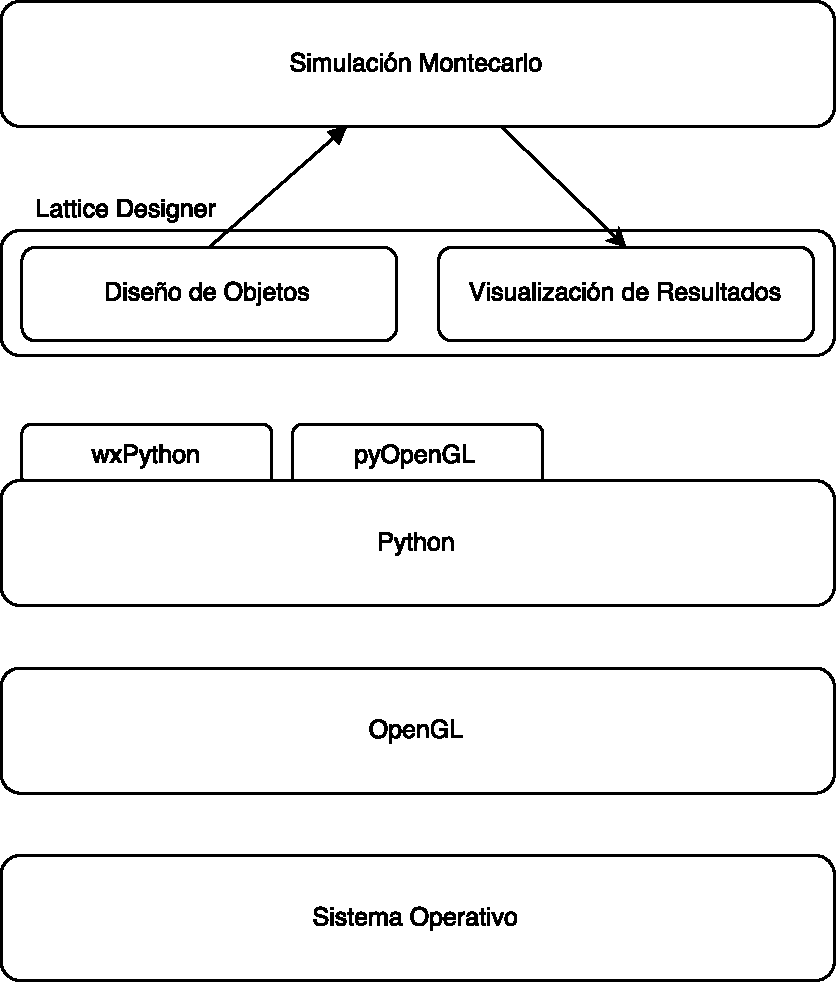
\includegraphics[scale=.7]{images/arquitectura}
  \caption{\em Diagrama de la arquitectura de la solución.}
  \label{arquitectura}
\end{figure}

\section{Sistema Operativo}

Si bien la aplicación fue desarrollada íntegramente en Mac OS X, y es por lo tanto el sistema operativo oficial de la presente memoria, todo el sistema fue desarrollado pensando en ser eventualmente multi-plataforma, sin que esta portación a distintos Sistemas Operativos tenga mayores complicaciones, más allá de los problemas que uno pueda encontrar por la distinta estructura de estos. Para esto tanto la elección del lenguaje de programación como de las distintas bibliotecas usadas fueron hechas teniendo el cuenta que deben poder ser ejecutados en los 3 sistemas operativos más usados, OS X, Windows y Linux.

\section{OpenGL}

Como parte importante del software es su capacidad de representar gráficamente en 3D tanto los átomos de un objeto diseñado como los resultados de las simulaciones, es necesario buscar una biblioteca de procesamiento gráfico 3D que fuera realmente multi-plataforma, tanto a nivel de sistema operativo como de tarjetas gráficas. Debido a esto se elige el estándar OpenGL, el cuál tiene implementaciones tanto para Windows, OS X y Linux, además de ser el estándar de la industria para gráficos 2D y 3D \citep{website:AboutOpenGL}. Esto permite tener una gran comunidad activa lo que a su vez se traduce en una gran cantidad de documentación al respecto.

La especificación del estándar OpenGL era dirigido por el consorcio independiente \emph{OpenGL Architecture Review Board} hasta el año 2006, cuando se decidió transferir esta responsabilidad al \emph{Khronos Group} \citep{website:OpenGLARB}, un consorcio formado por distintas organizaciones, tanto empresariales como académicas, quienes manejan múltiples estándares de la industria como \emph{OpenGL ES}, \emph{OpenCL} y \emph{WebGL} \citep{website:KhronosGroup}.

\section{Python}

Para el lenguaje de programación se barajó inicialmente la opción de C++ por las ventajas que conlleva trabajar a bajo nivel. No obstante debido a su inclinada curva de aprendizaje y complejidad he decidido usar Python, ya que es un lenguage que también cumple con las características necesarias para este desarrollo, como el ser multi-plataforma, y tener a disposición bibliotecas de manejo gráfico como su compatibilidad con la API OpenGL, de tal forma de centrar la complejidad del proyecto en las representaciones 3D.

Python es un lenguaje de programación de alto nivel, interpretado y orientado a objetos, desarrollado durante el año 1990 por Guido van Rossum, aunque actualmente es de código abierto y mantenido por su comunidad, la que es liderada por la \emph{Python Software Foundation}, quienes además resguardan los derechos de este.

Algunas de las características más conocidas de Python es su fácil sintaxis y su gran biblioteca estándar, la que cubre áreas como Protocolos de comunicación, Ingeniería de software e Interfaces de Sistema Operativo \citep{pythonFeatures}.

Durante el desarrollo se la aplicación se usaron distintas bibliotecas, siendo las dos más importantes wxPython y pyOpenGL.

\subsection{wxPython}

wxPython es una biblioteca de python que permite usar de forma nativa wxWidgets, un set de herramientas de código abierto, escrita en C++ y inicialmente escrito por Julian Smart y actualmente mantenida por la comunidad que permiten crear interfaces gráficas en distintas plataformas como Windows, OS X, iOS, Linux, entre otros. En este trabajo wxPython maneja todas las interacciones de los usuarios, además de casi todas las interfaces gráficas con excepción de los \emph{canvas} de OpenGL.

\subsection{pyOpenGL}

pyOpenGL es una biblioteca que permite la programación en OpenGL directamente desde python. Es multiplataforma y totalmente compatible con la biblioteca de interfaz gráfica usada (wxPython). Uno de los sub-paquetes de pyOpenGL usado en esta memoria es GLUT, la que permite crear fácilmente ciertos objetos en OpenGL, como esferas o conos, de tal forma de no tener que programar estos a partir de triángulos, como sería si se usara OpenGL puro.

\section{Lattice Designer}

Lattice Designer es el software desarrollado en esta memoria, el cual permite a científicos generar configuraciones atómicas sobre los cuales se simula la aplicación de campos electromagnéticos y la visualización de resultados generados por la simulación. Aunque esta herramienta está pensada para ser usada por investigadores del Departamento de Física de la Universidad de Santiago de Chile, la aplicación que ejecuta la simulación es usada por diversas organizaciones académicas, por lo que este software pretende ser un aporte a la comunidad científica en general.

Durante el desarrollo se puso especial énfasis en la experiencia de usuario, de tal forma que cualquier científico que tenga acceso a esta aplicación sea capaz de usarlo sin la necesidad de un entrenamiento; por este motivo el software tiene todos sus textos en inglés.

Como lo muestra la figura \ref{arquitectura}, la aplicación se compone de dos módulos claramente definidos: el diseño de configuraciones atómicas y la visualización de resultados de la simulación Monte Carlo.

\subsection{Diseño de configuraciones atómicas}

Para el desarrollo de esta funcionalidad se usó como base el sistema de diseño de objetos actual, basado en un mapa de bits, explicado en la sección \ref{intro:procesoactualmapa} de esta memoria, pero con la finalidad de que el proceso completo sea ejecutado en la misma aplicación disminuyendo con esto la probabilidad de errores que se puedan producir.

Dentro de las entradas de esta funcionalidad están tanto el mapa de bits, mediante una grilla binaria, como los distintos parámetros físicos asociados al objeto, como el tipo de estructura cristalina, la constante de red y el número de capas, entre otros (ver figura \ref{softwareDiseno}). Además se le ofrece al usuario mucha información dinámica, es decir, que va cambiando en base a los parámetros de entrada, como por ejemplo la constante de escalamiento.

\begin{figure}[ht]
  \centering
  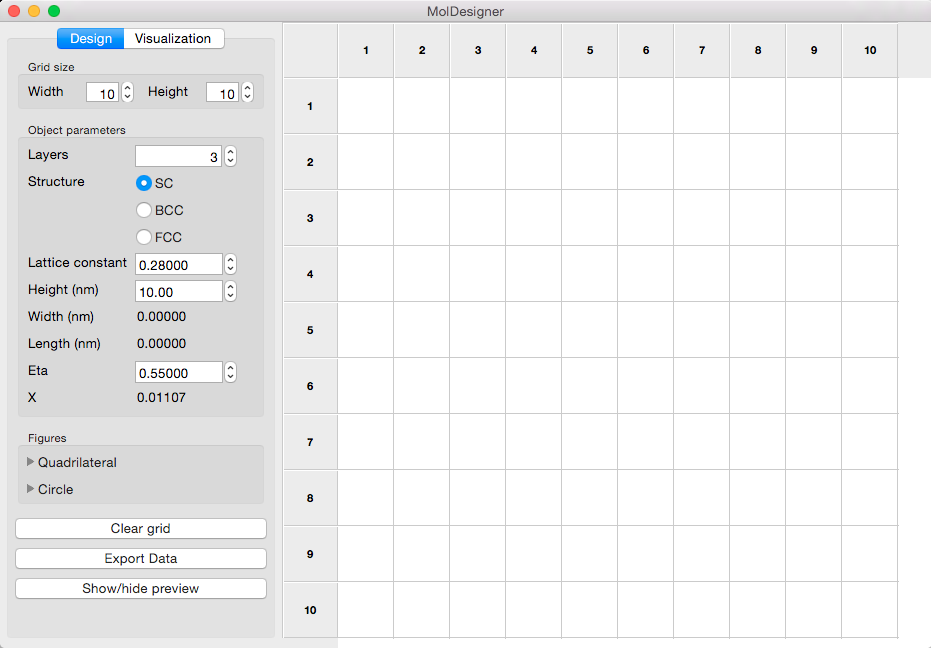
\includegraphics[scale=.45]{images/softwareDiseno}
  \caption{\em Vista de diseño de configuraciones atómicas del software}
  \label{softwareDiseno}
\end{figure}

Una de las características del diseño es la posibilidad de crear imágenes pre-definidas en base a dimensiones entregadas por el usuario. De esta forma se pueden crear cuadriláteros definiendo su ancho y alto o circunferencias con un radio específico. Una vez ingresados los parámetros solo es necesario hacer click en la posición de la grilla donde se quiere dibujar.

Como muestra la figura \ref{softwareDisenoPrevisualizacion}, el software permite también al usuario ver de forma inmediata la visualización 3D de la configuración atómica que se está creando con colores identificando sus distintos tipos de partículas, permitiendo así comprobar de manera rápida y fácil si efectivamente el diseño es el deseado.

\begin{figure}[ht]
  \centering
  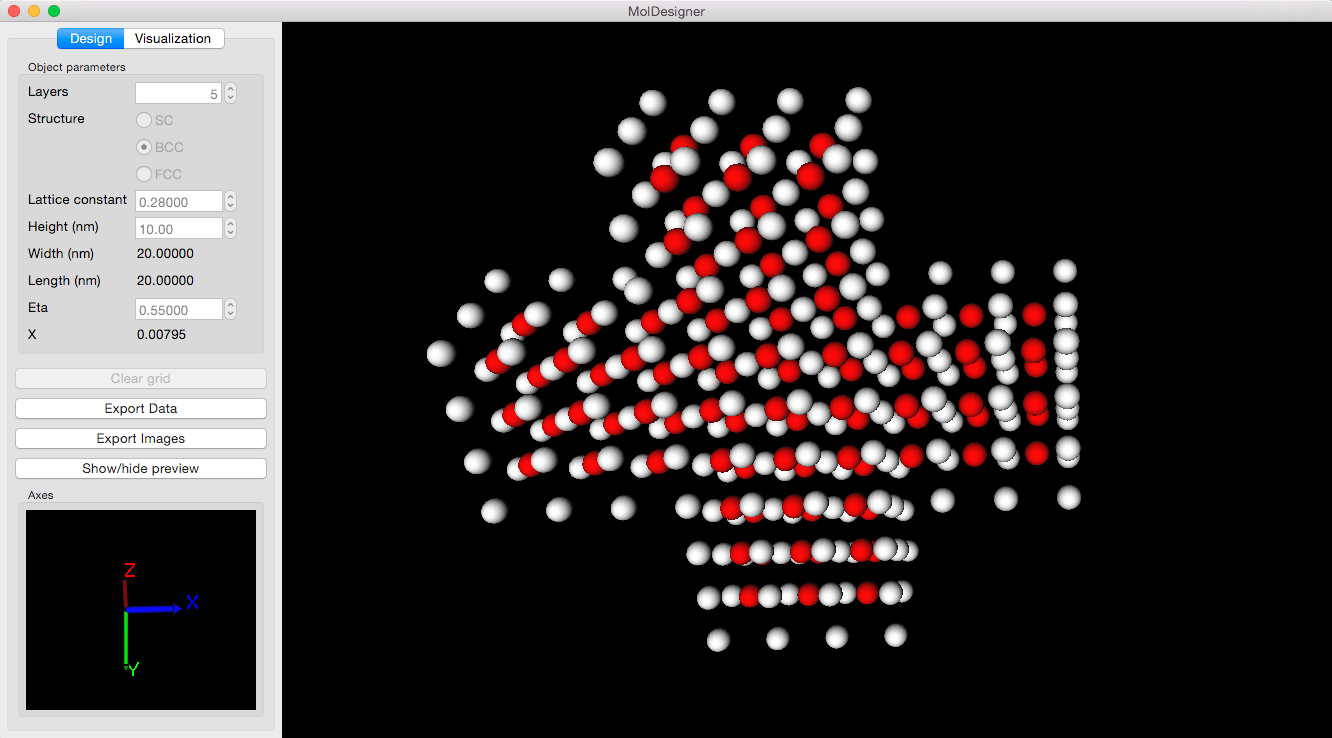
\includegraphics[scale=.35]{images/softwareDisenoPrevisualizacion}
  \caption{\em Previsualización de un objeto diseñado}
  \label{softwareDisenoPrevisualizacion}
\end{figure}

Una vez confirmado que el objeto diseñado es el deseado es posible exportar directamente las imágenes de la configuración atómica y los ejes coordenados para referencia; así como también el archivo que describe la configuración atómica, el que sirve como entrada para el software de simulación. A diferencia del proceso actual, donde el archivo exportado debe ser modificado para poder ser usado, en este caso los datos exportados puedes ser usados inmediatamente para ejecutar una simulación.

\subsection{Visualización de resultados}

El segundo módulo se basa específicamente en los requerimientos de los \emph{stakeholders}, sin tener un proceso actual como base, ya que esta es la gran debilidad que tienen actualmente.

Dentro de las funcionalidades de este módulo se encuentra la visualización y exportación del estado de la simulación en un tiempo \emph{t}, incluyendo los vectores de campo magnético, la curva de histéresis del campo magnético y los ejes coordenados para referencia. Estos son elementos que los científicos necesitan en sus publicaciones.

Las figuras \ref{softwareVisualizacionVectors}, \ref{softwareVisualizacionAxes} y \ref{softwareVisualizacionPlot} son las tres imágenes que se pueden exportar del estado de la simulación representado en la figura \ref{softwareVisualizacionPantalla}.


\begin{figure}[ht]
  \centering
  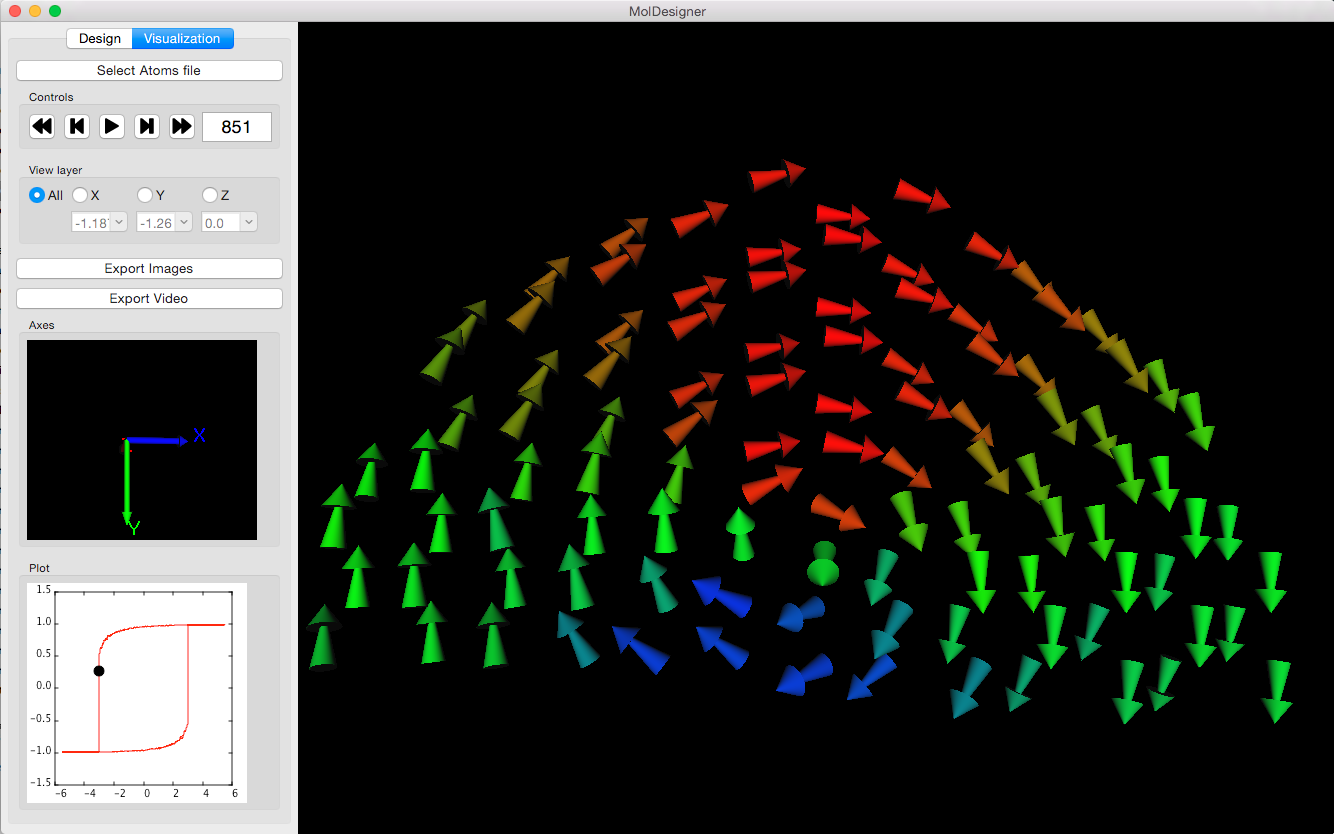
\includegraphics[scale=.3]{images/softwareVisualizacionPantalla}
  \caption{\em Pestaña de visualización de resultados en $t = 851$}
  \label{softwareVisualizacionPantalla}
\end{figure}


\begin{figure}[ht]
  \centering
  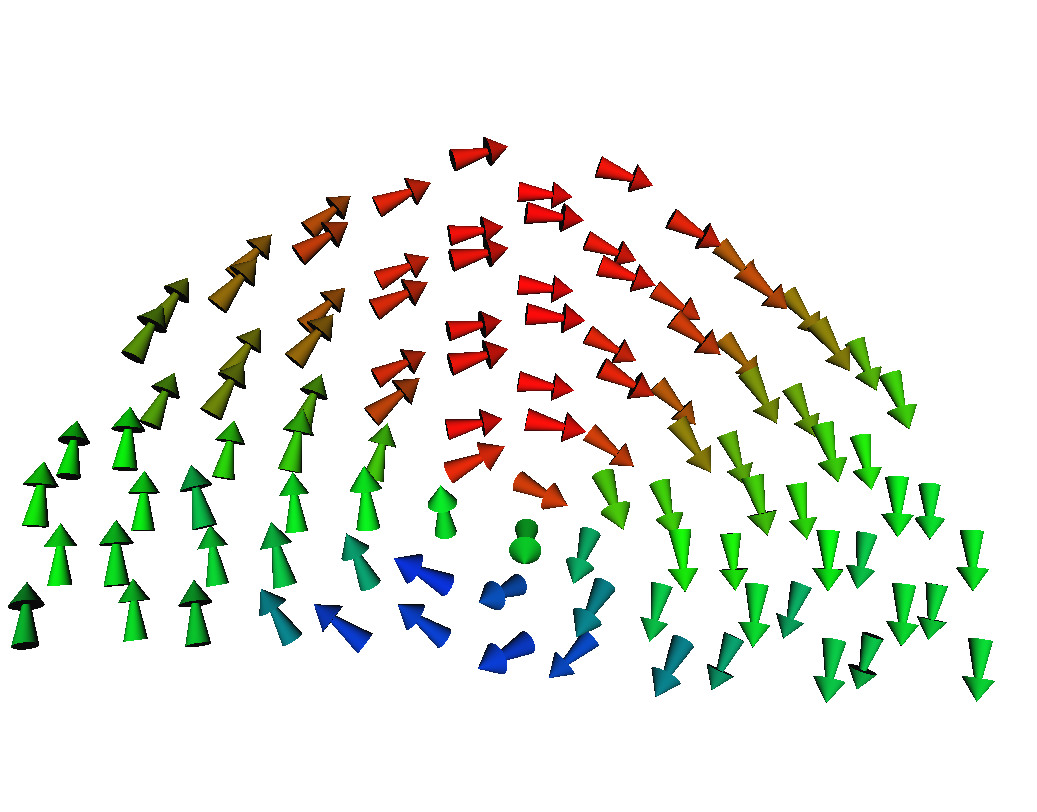
\includegraphics[scale=.3]{images/softwareVisualizacionVectors}
  \caption{\em Imagen de vectores exportada para publicación}
  \label{softwareVisualizacionVectors}
\end{figure}


\begin{figure}[ht]
  \centering
  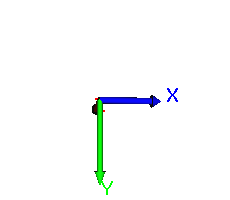
\includegraphics[scale=.6]{images/softwareVisualizacionAxes}
  \caption{\em Imagen de ejes de referencia exportada para publicación}
  \label{softwareVisualizacionAxes}
\end{figure}


\begin{figure}[ht]
  \centering
  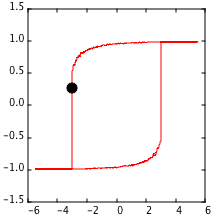
\includegraphics[scale=.6]{images/softwareVisualizacionPlot}
  \caption{\em Imagen de curva de histéresis exportada para publicación}
  \label{softwareVisualizacionPlot}
\end{figure}

Otras características disponibles es la asignación de colores para cada vector según uno de sus componentes cartesianos, usando una escala de colores de azul a rojo. En el caso de la figura \ref{softwareVisualizacionVectors} el máximo valor de $\hat{i}$ será rojo y el mínimo será azul. Esto permite identificar rápidamente una tercera dimensión en una imagen 2D y también los vortex que se generan.

También es posible ver la variación de los vectores a través del tiempo como video y luego exportarlo de tal forma que este pueda ser usado fácilmente en conferencias donde se divulguen los resultados.

Cabe notar que todas las características anteriores pueden ser ejecutadas mientras se visualiza solo una de las múltiples capas en la que se puede dividir el objeto, en base a cualquier eje coordenado, como se puede ver en las figuras \ref{softwareVisualizacionVectorsZ} y \ref{softwareVisualizacionVectorsX}.

\begin{figure}[ht]
  \centering
  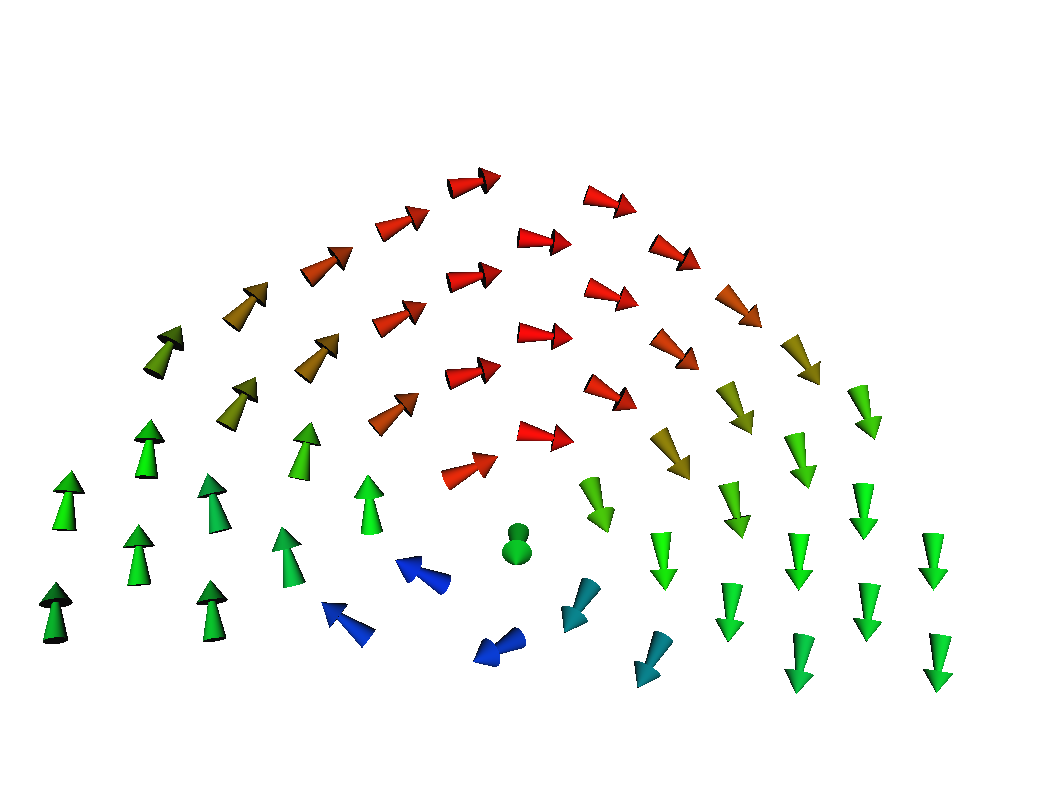
\includegraphics[scale=.3]{images/softwareVisualizacionVectorsZ}
  \caption{\em Estado de la simulación para t = 851 solo para la capa Z = 0}
  \label{softwareVisualizacionVectorsZ}
\end{figure}


\begin{figure}[ht]
  \centering
  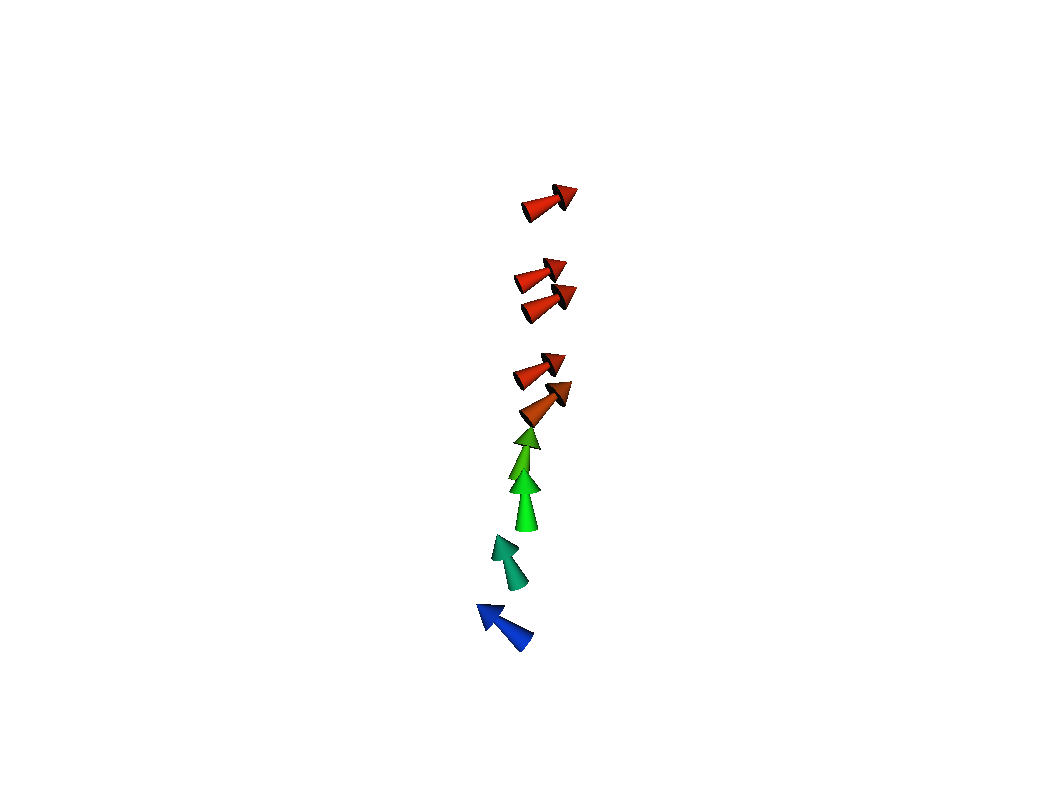
\includegraphics[scale=.3]{images/softwareVisualizacionVectorsX}
  \caption{\em Estado de la simulación para t = 851 solo para la capa X = -0.395}
  \label{softwareVisualizacionVectorsX}
\end{figure}
\chapter{Implementación de la solución}
\label{chapter:implementacion}

\section{Clases}

Para el desarrollo de la aplicación se usó el lenguaje Python, dividiendo la aplicación en clases que se pueden categorizar de la siguiente forma:

\subsection{Clases visuales}

\subsubsection{LatticeDesigner}
Esta es la clase principal de la aplicación, ya que es la encargada de iniciar el programa, cargando todas las dependencias necesarias para su ejecución, pero principalmente implementa la lógica de la parte visual del \emph{software}, es decir, de la creación y distribución en pantalla de los distintos elementos visuales, como ventanas, botones, campos de texto, etc., además de la interacción del usuario con estos. Cada reacción a una acción ejecutada sobre estos elementos es orquestada por esta clase.

\subsubsection{BitmapGrid}
La clase BitmapGrid es la encargada de manejar la grilla con la cuales los científicos diseñarán las configuraciones atómicas que se simularán. Para esto se basa en la biblioteca \emph{wx.grid} de \emph{wxPython}, una implementación de una planilla de cálculos tipo \emph{excel}, la cual es modificada para no poder ser editada y que las distintas acciones del \emph{mouse} sobre esta (click, seleccionar fila o columna, seleccionar un rango de celdas, etc.) generen cambios en el color de fondo de cada celda, pudiendo este ser negro o blanco, transformando esta planilla de cálculos en un mapa de bits binario.

Entre las características de este mapa de bits se encuentra la capacidad de crear figuras predefinidas rápidamente. Por ejemplo, se puede dibujar un cuadrilátero indicando el ancho, el alto y seleccionando la esquina superior derecha de esta figura. También es posible crear un círculo indicando el radio que tendrá este y su centro. Estas dos figuras predefinidas pueden combinarse para crear configuraciones más complejas, como un elipsoide, que son de mucha utilidad para los científicos (ver figura \ref{elipsoide}).

\begin{figure}[ht]
  \centering
  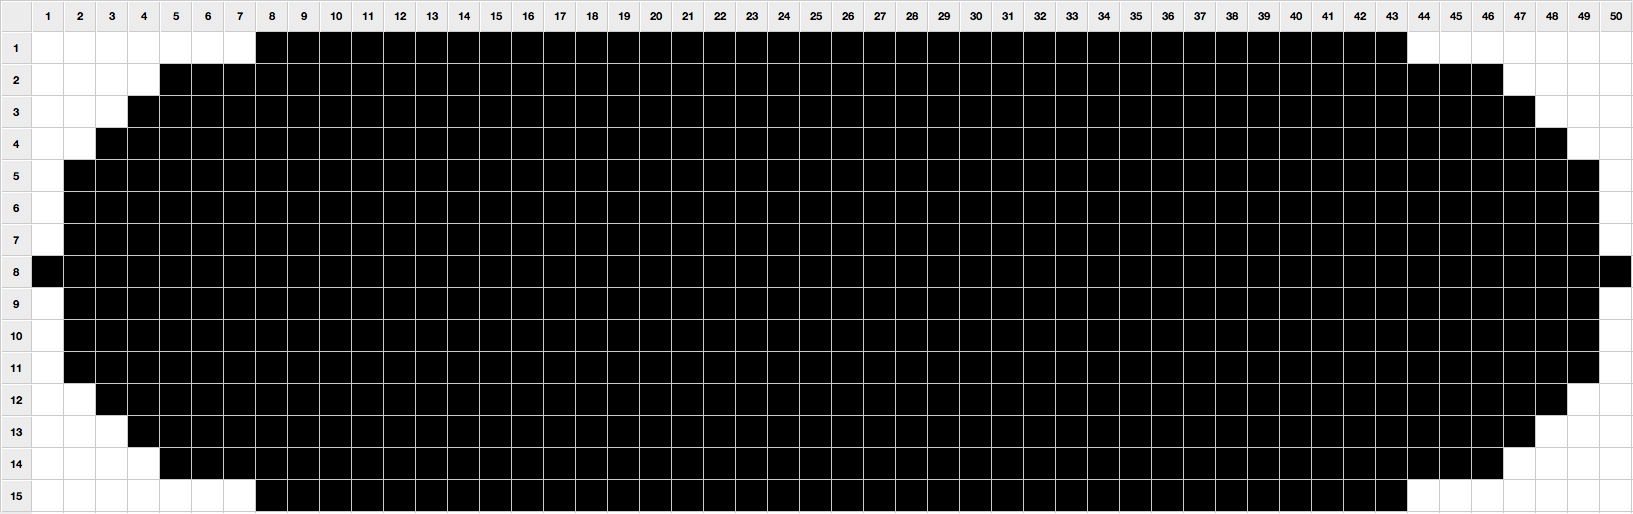
\includegraphics[scale=.25]{images/elipsoide}
  \caption{\em Mapa de bits binario con 2 figuras pre-diseñadas.}
  \label{elipsoide}
\end{figure}

\subsection{Clases 3D}

Estas clases son las encargadas de manejar los distintos \emph{canvas} que se usan en el \emph{software}, tanto para la visualización del diseño y del resultado de la simulación, como para ayudas referenciales para los científicos.

\subsubsection{AtomCanvas}

La clase AtomCanvas es la más importante con respecto a la visualización 3D, ya que es la encargada de mostrar en pantalla tanto el diseño de los objetos sobre los cuales se correrá la simulación como los resultados de estas usando OpenGL. En el desarrollo de esta clase se puso énfasis en la optimización, pudiendo mostrar sin mayores demoras más de 20.000 átomos. Para tener una idea un sistema promedio escalado analizado por los científicos usa 3.000 átomos (TODO: CONFIRMAR).

Otra de las tareas de esta clase es manejar las distintas interacciones del usuario, tanto con el teclado como con el \emph{mouse} con las representaciones en 3D, como rotaciones, movimientos y \emph{zoom}.

Para la visualización del diseño se usan esferas de distintos colores, representando cada uno de los distintos tipos de átomos que pueden haber según la estructura cúbica elegida. En las figuras \ref{atomCanvas-SC}, \ref{atomCanvas-BCC} y \ref{atomCanvas-FCC} se representan una estructura de 5x5 átomos, con 3 capas, siendo diferente solo la estructura cristalina elegida.

\begin{figure}[ht]
  \centering
  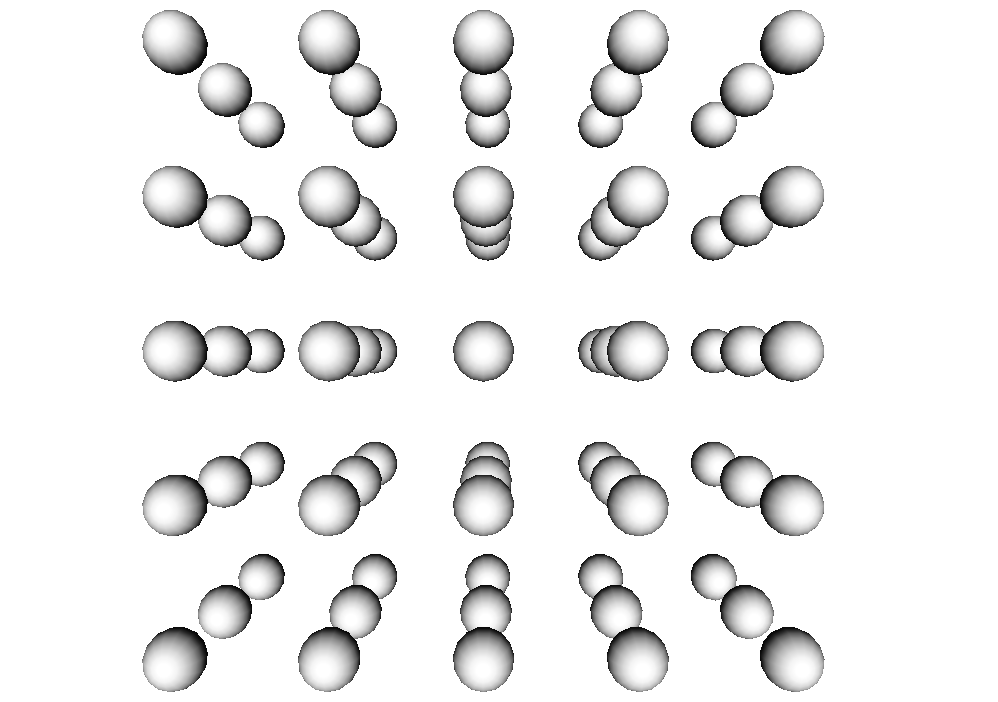
\includegraphics[scale=.3]{images/atomCanvas-SC}
  \caption{\em En un SC todos los átomos son blancos.}
  \label{atomCanvas-SC}
\end{figure}

\begin{figure}[ht]
  \centering
  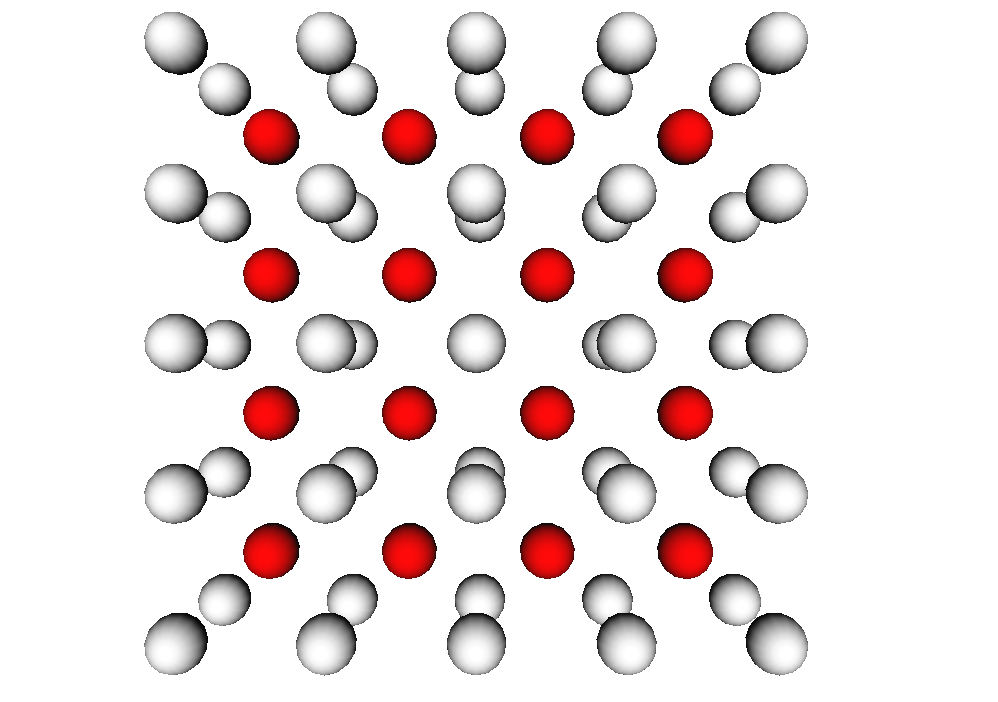
\includegraphics[scale=.3]{images/atomCanvas-BCC}
  \caption{\em En un BCC los átomos centrales son rojos.}
  \label{atomCanvas-BCC}
\end{figure}

\begin{figure}[ht]
  \centering
  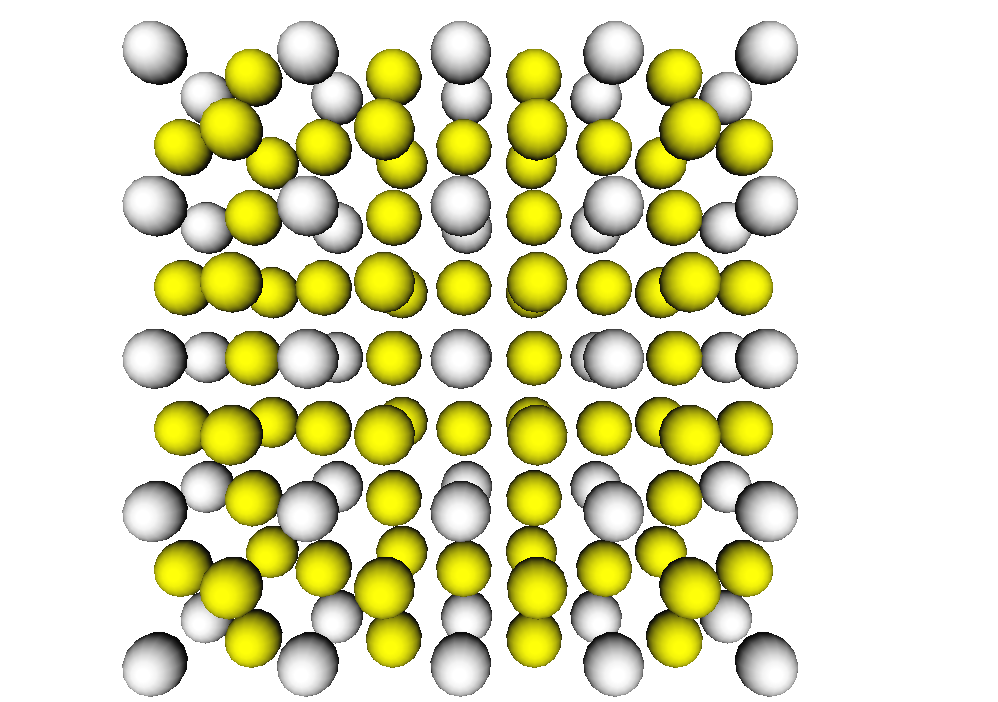
\includegraphics[scale=.35]{images/atomCanvas-FCC}
  \caption{\em En un FCC los átomos de las caras son amarillos.}
  \label{atomCanvas-FCC}
\end{figure}

En el caso de la visualización de resultados se usan flechas de colores como representación del momento magnético. Para asignar un color a una flecha se parte de la premisa que en tiempo t=0 el campo magnético externo está siendo aplicado hacia un eje, y por lo tanto inicialmente todos los vectores tendrán la misma magnitud, sentido y dirección, paralelos al campo externo, como se puede notar en la figura \ref{atomCanvas-vectores-inicial}. Además se sabe que en ese momento su magnitud es máxima. Si inicialmente todos los vectores son paralelos al eje A, se usa la componente â de cada vector para definir el color. Si la componente es 0 entonces será de color verde; si la magnitud es máxima en sentido contrario a los vectores iniciales el color será azul; si la magnitud es máxima en el mismo sentido de los vectores iniciales el color será rojo. Como se puede inferir la escala va desde azul a rojo, siendo este último color el inicial para todos los vectores. En la figura \ref{atomCanvas-vectores-colores} se puede ver los distintos colores según la componente $\hat{i}$ de los vectores, dado que el campo externo inicial tiene sentido $[1, 0, 0]$.

\begin{figure}[ht]
  \centering
  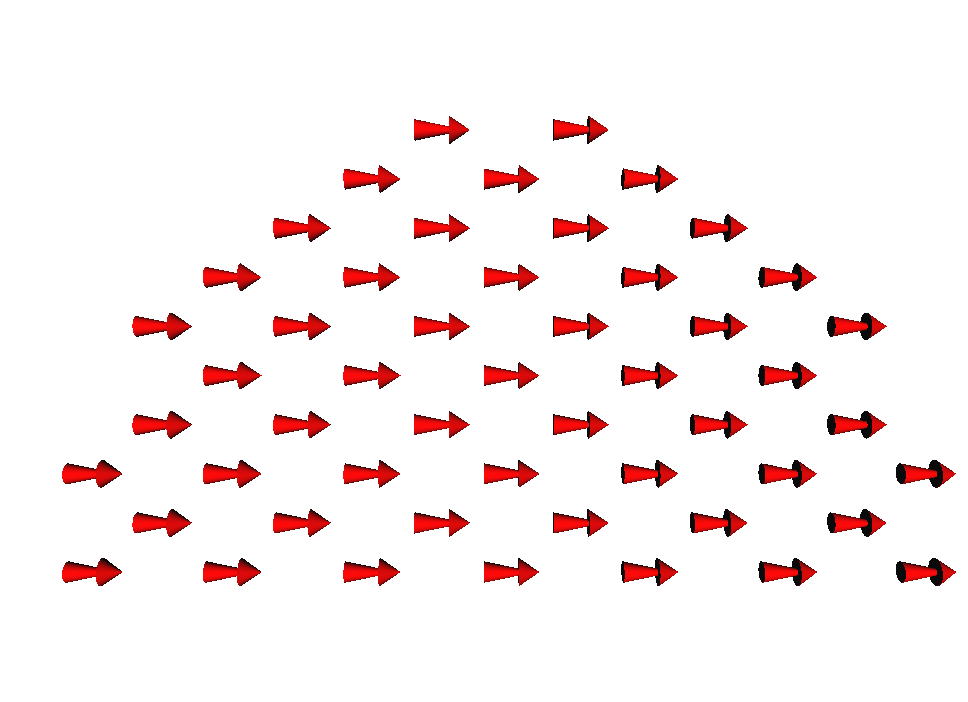
\includegraphics[scale=.3]{images/atomCanvas-vectores-inicial}
  \caption{\em Estado inicial de la visualización, con todos los vectores rojos paralelos al campo magnético externo inicial.}
  \label{atomCanvas-vectores-inicial}
\end{figure}

\begin{figure}[ht]
  \centering
  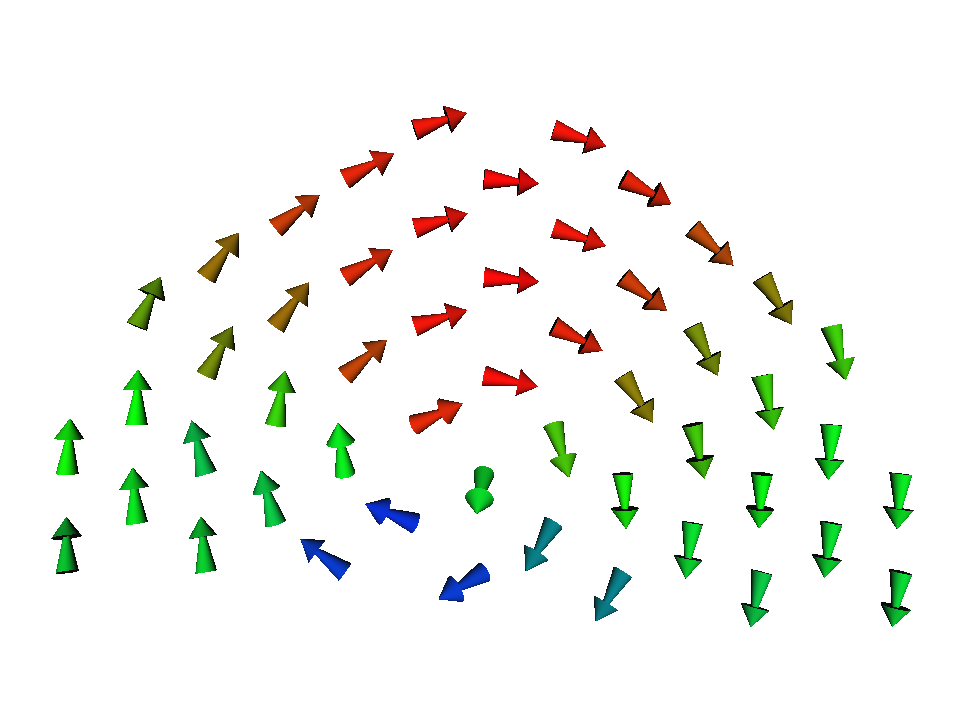
\includegraphics[scale=.3]{images/atomCanvas-vectores-colores}
  \caption{\em Vectores de distintos colores según la componente $\hat{i}$.}
  \label{atomCanvas-vectores-colores}
\end{figure}

\subsubsection{Axes}

La clase Axes es la encargada de mostrar los ejes coordenados de los distintos canvas, tanto del de diseño de objetos como el de visualización de resultados, usando Open GL.
Cada eje se representa con su propio color, usando azul, rojo y verde para los ejes X, Y y Z respectivamente, y una etiqueta con el mismo color, de forma de hacerlo fácil de visualizar para el usuario.
Debido al diseño del \emph{software}, donde las distintas funciones del programa (diseño y visualización) se seleccionan mediante pestañas, esta clase debe ser instanciada 2 veces, ya que no es posible usar la misma instancia en ambas secciones. Estas se comunican directamente con AtomCanvas para obtener los distintos parámetros de rotación de forma que los ejes sean coherentes a la imagen mostrada.

\begin{figure}[ht]
  \centering
  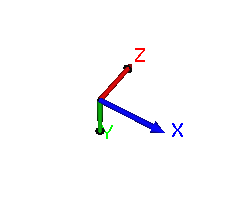
\includegraphics[scale=1]{images/axes}
  \caption{\em Representación visual de los ejes coordenados.}
\end{figure}

\subsection{Clases de cubos}


Las clases de cubos son 3 clases (\emph{SC}, \emph{BCC} y \emph{FCC}) que heredan de un mismo padre, \emph{Cube}. Estas crean los átomos de un objeto que se está diseñando. Las 3 clases hermanas tienen solo 2 métodos: \emph{calculate} y \emph{find\_neighborhood}. El primero se encarga de identificar todos los átomos que conforman la configuración atómica, dados los parámetros físicos como la estructura de la primera capa. El segundo define cuales son los parámetros para llamar al método \emph{find\_neighborhood} de la súper clase, el que busca todos los vecinos inmediatos para cada átomo. Estos parametros son necesarios para exportar el archivo que luego servirá de entrada para la simulación.

\subsubsection{Cube}
TBD


\subsubsection{SC}
SC es la clase que maneja los cubos simples (\emph{Simple Cubic} o \emph{SC}), estas estructuras cúbicas se caracterizan por tener un átomo en cada uno de sus vértices, por lo que la identificación de sus átomos se reduce a simplemente repetir la capa superior tantas veces como sea indicado en la entrada de propiedades físicas. Para encontrar el vecindario es necesario buscar todos los átomos que estén en las siguientes posiciones relativas [-1,0,0], [1,0,0], [0,-1,0], [0,1,0], [0,0,-1] y [0,0,1], por lo que el tamaño máximo de su vecindad es de 6 átomos.

\subsubsection{BCC}
BCC es la clase que maneja los cubos centrados en el cuerpo (\emph{Body Centered Cubic} o \emph{BCC}), que son las estructuras cúbicas que además de tener un átomo en cada vértice de los cubos tienen uno en el centro de cada uno de estos. Esto implica que en la identificación de átomos se debe trabajar con una capa intermedia que contiene los centros de cada cubo. por ejemplo, para una estructura de 5 capas quedaría así:
\begin{center}
  \begin{tabular}{ c | l }
    \# & Capa \\
    \hline
    1 & Primaria \\
    2 & Intermedia \\
    3 & Primaria \\
    4 & Intermedia \\
    5 & Primaria \\
    \hline
  \end{tabular}
\end{center}

La regla para agregar un átomo central es que debe tener un cubo de átomos a su alrededor, y en caso que el cubo no esté completo simplemente se usan las capas primarias, como se puede notar en las figuras \ref{BCC-incomplete-molecule} y \ref{BCC-complete-molecule}.

\begin{figure}[ht]
  \centering
  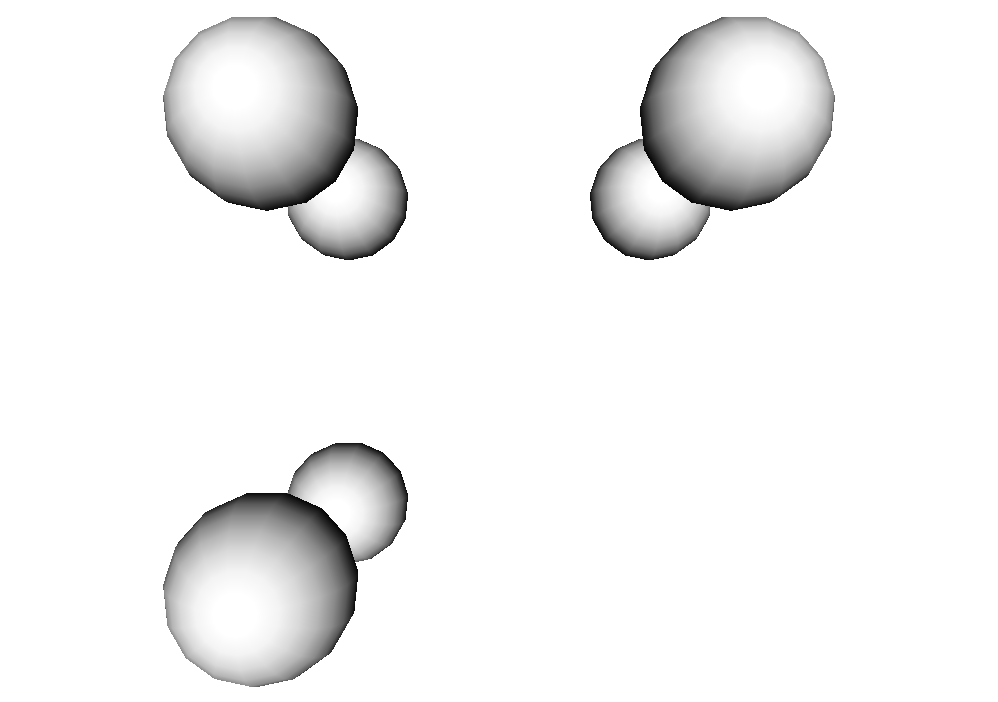
\includegraphics[scale=.3]{images/BCC-incomplete-molecule}
  \caption{\em Cubo BCC incompleto, sin átomo central}
  \label{BCC-incomplete-molecule}
\end{figure}

\begin{figure}[ht]
  \centering
  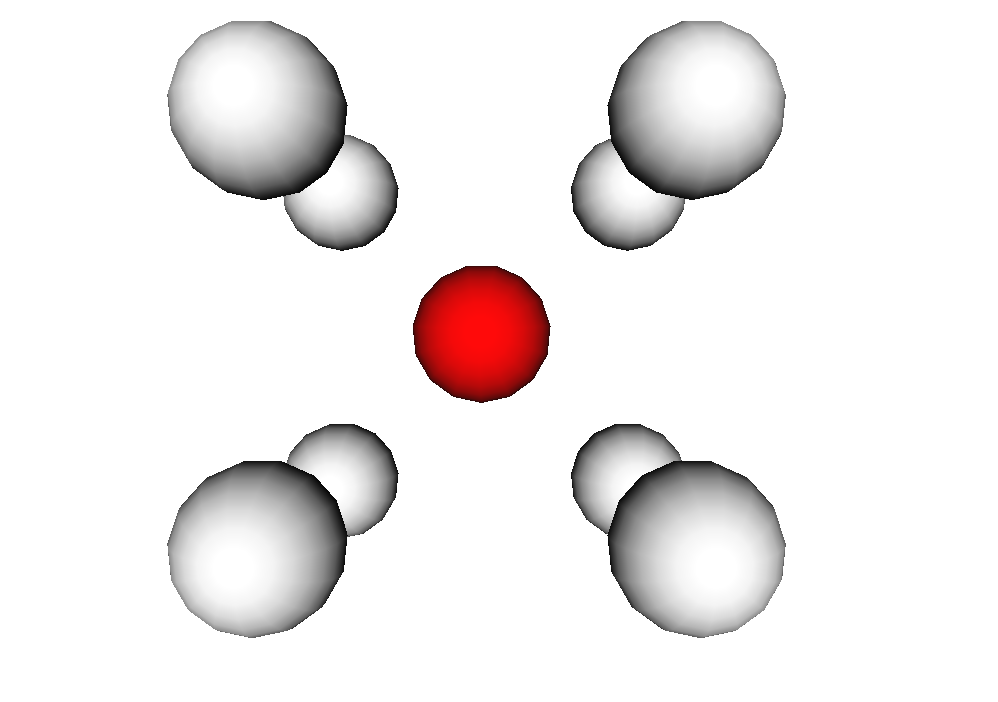
\includegraphics[scale=.3]{images/BCC-complete-molecule}
  \caption{\em Cubo BCC completo, con átomo central}
  \label{BCC-complete-molecule}
\end{figure}

En el caso de los BCC los átomos que conforman la vecindad siempre estarán en las posiciones relativas $[\pm 0.5, \pm 0.5, \pm 0.5]$, es decir, cada átomo puede tener una vecindad compuesta por hasta 8 átomos.

\subsubsection{FCC}
FCC es la clase que maneja los cubos centrados en las caras (\emph{Face Centered Cubic} o \emph{FCC}), los cuales se caracterizan por tener un átomo extra por cara además de uno en cada uno de sus vértices, por lo que además de tener que crear una capa intermedia es necesario modificar la capa primaria, es decir, la que crea el usuario usando el mapa de bits. La regla para agregar estos átomos en las caras es que ellos estén en la diagonal creada por otros 2 átomos, en cualquier dirección. En la figura \ref{FCC-diagonal} se ve como en una estructura cúbica de 1x2, como en una de sus caras se forma una diagonal entre 2 átomos y por lo tanto es necesario agregar un átomo extra en una capa intermedia.

\begin{figure}[ht]
  \centering
  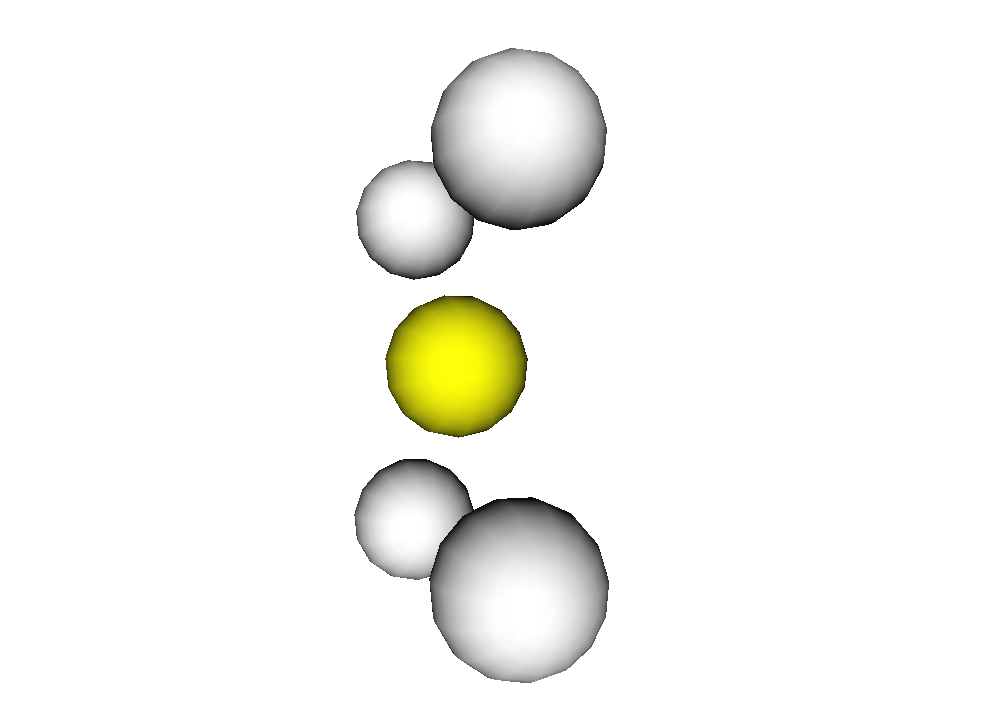
\includegraphics[scale=.3]{images/FCC-diagonal}
  \caption{\em Estructura cúbica FCC, con átomo en una de sus caras}
  \label{FCC-diagonal}
\end{figure}

La vecindad de estas estructuras cúbicas está dada por la posición relativa dada por $[\alpha, \beta, \gamma]$, donde:

\[
	\begin{cases}
		$$(\alpha = \pm 0.5; \beta = \pm 0.5; \gamma = 0)$$ \\
		$$(\alpha = \pm 0.5; \beta = 0; \gamma = \pm 0.5)$$ \\
		$$(\alpha = 0; \beta = \pm 0.5; \gamma = \pm 0.5)$$
	\end{cases}
\]
% 		$n/2 & \quad \text{if } n \text{ is even}\\ -(n+1)/2 & \quad \text{if } n \text{ is odd}\\ 

% $$  \vee  \vee $$

Lo que resulta en 12 posiciones posibles, siendo este el número máximo de átomos en una vecindad.




% ----------------------------------------------------------
% ----------- TERCERA PARTE --------------------------------
% \backmatter %Elimina la numeración
% ### Bibliografía de este documento ###
\bibliographystyle{apa-good}
\bibliography{referencias}
% ----------------------------------------------------------
% ----------- CUARTA PARTE ---------------------------------
\appendix
\addappheadtotoc %agregar Apéndice al índice. Si no tiene apéndices COMENTAR o BORRAR
% \noappendicestocpagenum %quitar número de páginas a los apéndices
% ### APENDICES ###
%\fontsize{9}{10.8} %tamaño de letra para apendices es 9pt
\linespread{1.0} %interlineado de 1 para los apéndices
\small %tamaño 9 para los apéndices


\chapter{Manual de usuario}
\label{cap:manual}

%DESCOMENTAR ESTAS LINEAS SI EL CAPÍTULO TIENE FIGURAS O TABLAS
%\addtocontents{lof}{{\bf \noindent Figuras del Anexo \Alph{chapter}}}
\addtocontents{lot}{{\bf \noindent Tablas del Anexo \Alph{chapter}}}

\section{Requerimientos previos}

\subsection{Requerimientos para instalación}
blablabla

\begin{table}[ht]
\caption{Tabla que dice nada}\label{tab:nombreTablaReferenciable}
\small %hace que el contenido de las tablas tengan tamaño 9
\centering
\begin{tabular}{lll}
Animal    & Description & Price (\$) \\
\hline
Gnat      & per gram    & 13.65      \\
          & each        & 0.01       \\
Gnu       & stuffed     & 92.50      \\
Emu       & stuffed     & 33.33      \\
Armadillo & frozen      & 8.99       \\
\hline
\end{tabular}
\end{table}
 % Manuales de Usuario
%\include{apendices/Apendice-2} % Eventos
%\include{apendices/Apendice-3} % Clases
%\include{apendices/Apendice-4} % Peticiones HTTP y objetos transferidos
%\include{apendices/Apendice-5} % Uso de memoria
%\include{apendices/Apendice-6} % Archivos de entrada
%\include{apendices/Apendice-7} % Código fuente de ejemplo de aplicación concreta
\end{document}
%\\end